\documentclass[english,11pt]{beamer}

\DeclareMathOperator{\Cov}{Cov}
\DeclareMathOperator{\Var}{Var}
\DeclareMathOperator{\E}{\mathbb{E}}
\DeclareMathOperator{\Proba}{\mathbb{P}}

\newcommand{\Covb}[2]{\ensuremath{\Cov\!\left[#1,#2\right]}}
\newcommand{\Eb}[1]{\ensuremath{\E\!\left[#1\right]}}
\newcommand{\Pb}[1]{\ensuremath{\Proba\!\left[#1\right]}}
\newcommand{\Varb}[1]{\ensuremath{\Var\!\left[#1\right]}}

% norm
\newcommand{\norm}[1]{\| #1 \|}

\newcommand{\indep}{\rotatebox[origin=c]{90}{$\models$}}





\usepackage{mathptmx,amsmath,amssymb,graphicx,bibentry,bbm,babel,ragged2e}

\makeatletter

\newcommand{\noun}[1]{\textsc{#1}}
\newcommand{\jitem}[1]{\item \begin{justify} #1 \end{justify} \vfill{}}
\newcommand{\sframe}[2]{\frame{\frametitle{#1} #2}}

\newenvironment{centercolumns}{\begin{columns}[c]}{\end{columns}}
%\newenvironment{jitem}{\begin{justify}\begin{itemize}}{\end{itemize}\end{justify}}

\usetheme{Warsaw}
\setbeamertemplate{footline}[text line]{}
\setbeamercolor{structure}{fg=purple!50!blue, bg=purple!50!blue}

\setbeamersize{text margin left=15pt,text margin right=15pt}

\setbeamercovered{transparent}


\@ifundefined{showcaptionsetup}{}{%
 \PassOptionsToPackage{caption=false}{subfig}}
\usepackage{subfig}

\usepackage[utf8]{inputenc}
\usepackage[T1]{fontenc}

\usepackage{multirow}


\makeatother

\begin{document}





\title{Développement de méthodes pour la validation des modèles d'interaction Transport-Usage du sol}

\author{OpenMOLE Team}


%\institute{$^{1}$Complex Systems Institute, Paris, UPS CNRS 3611 ISC-PIF\\
%$^{2}$UMR CNRS 8504 G{\'e}ographie-cit{\'e}s
%}


\date{ISCoffee Break\\
06/12/2018
}

\frame{\maketitle}



\sframe{Interactions entre réseaux et territoires}{

\centering

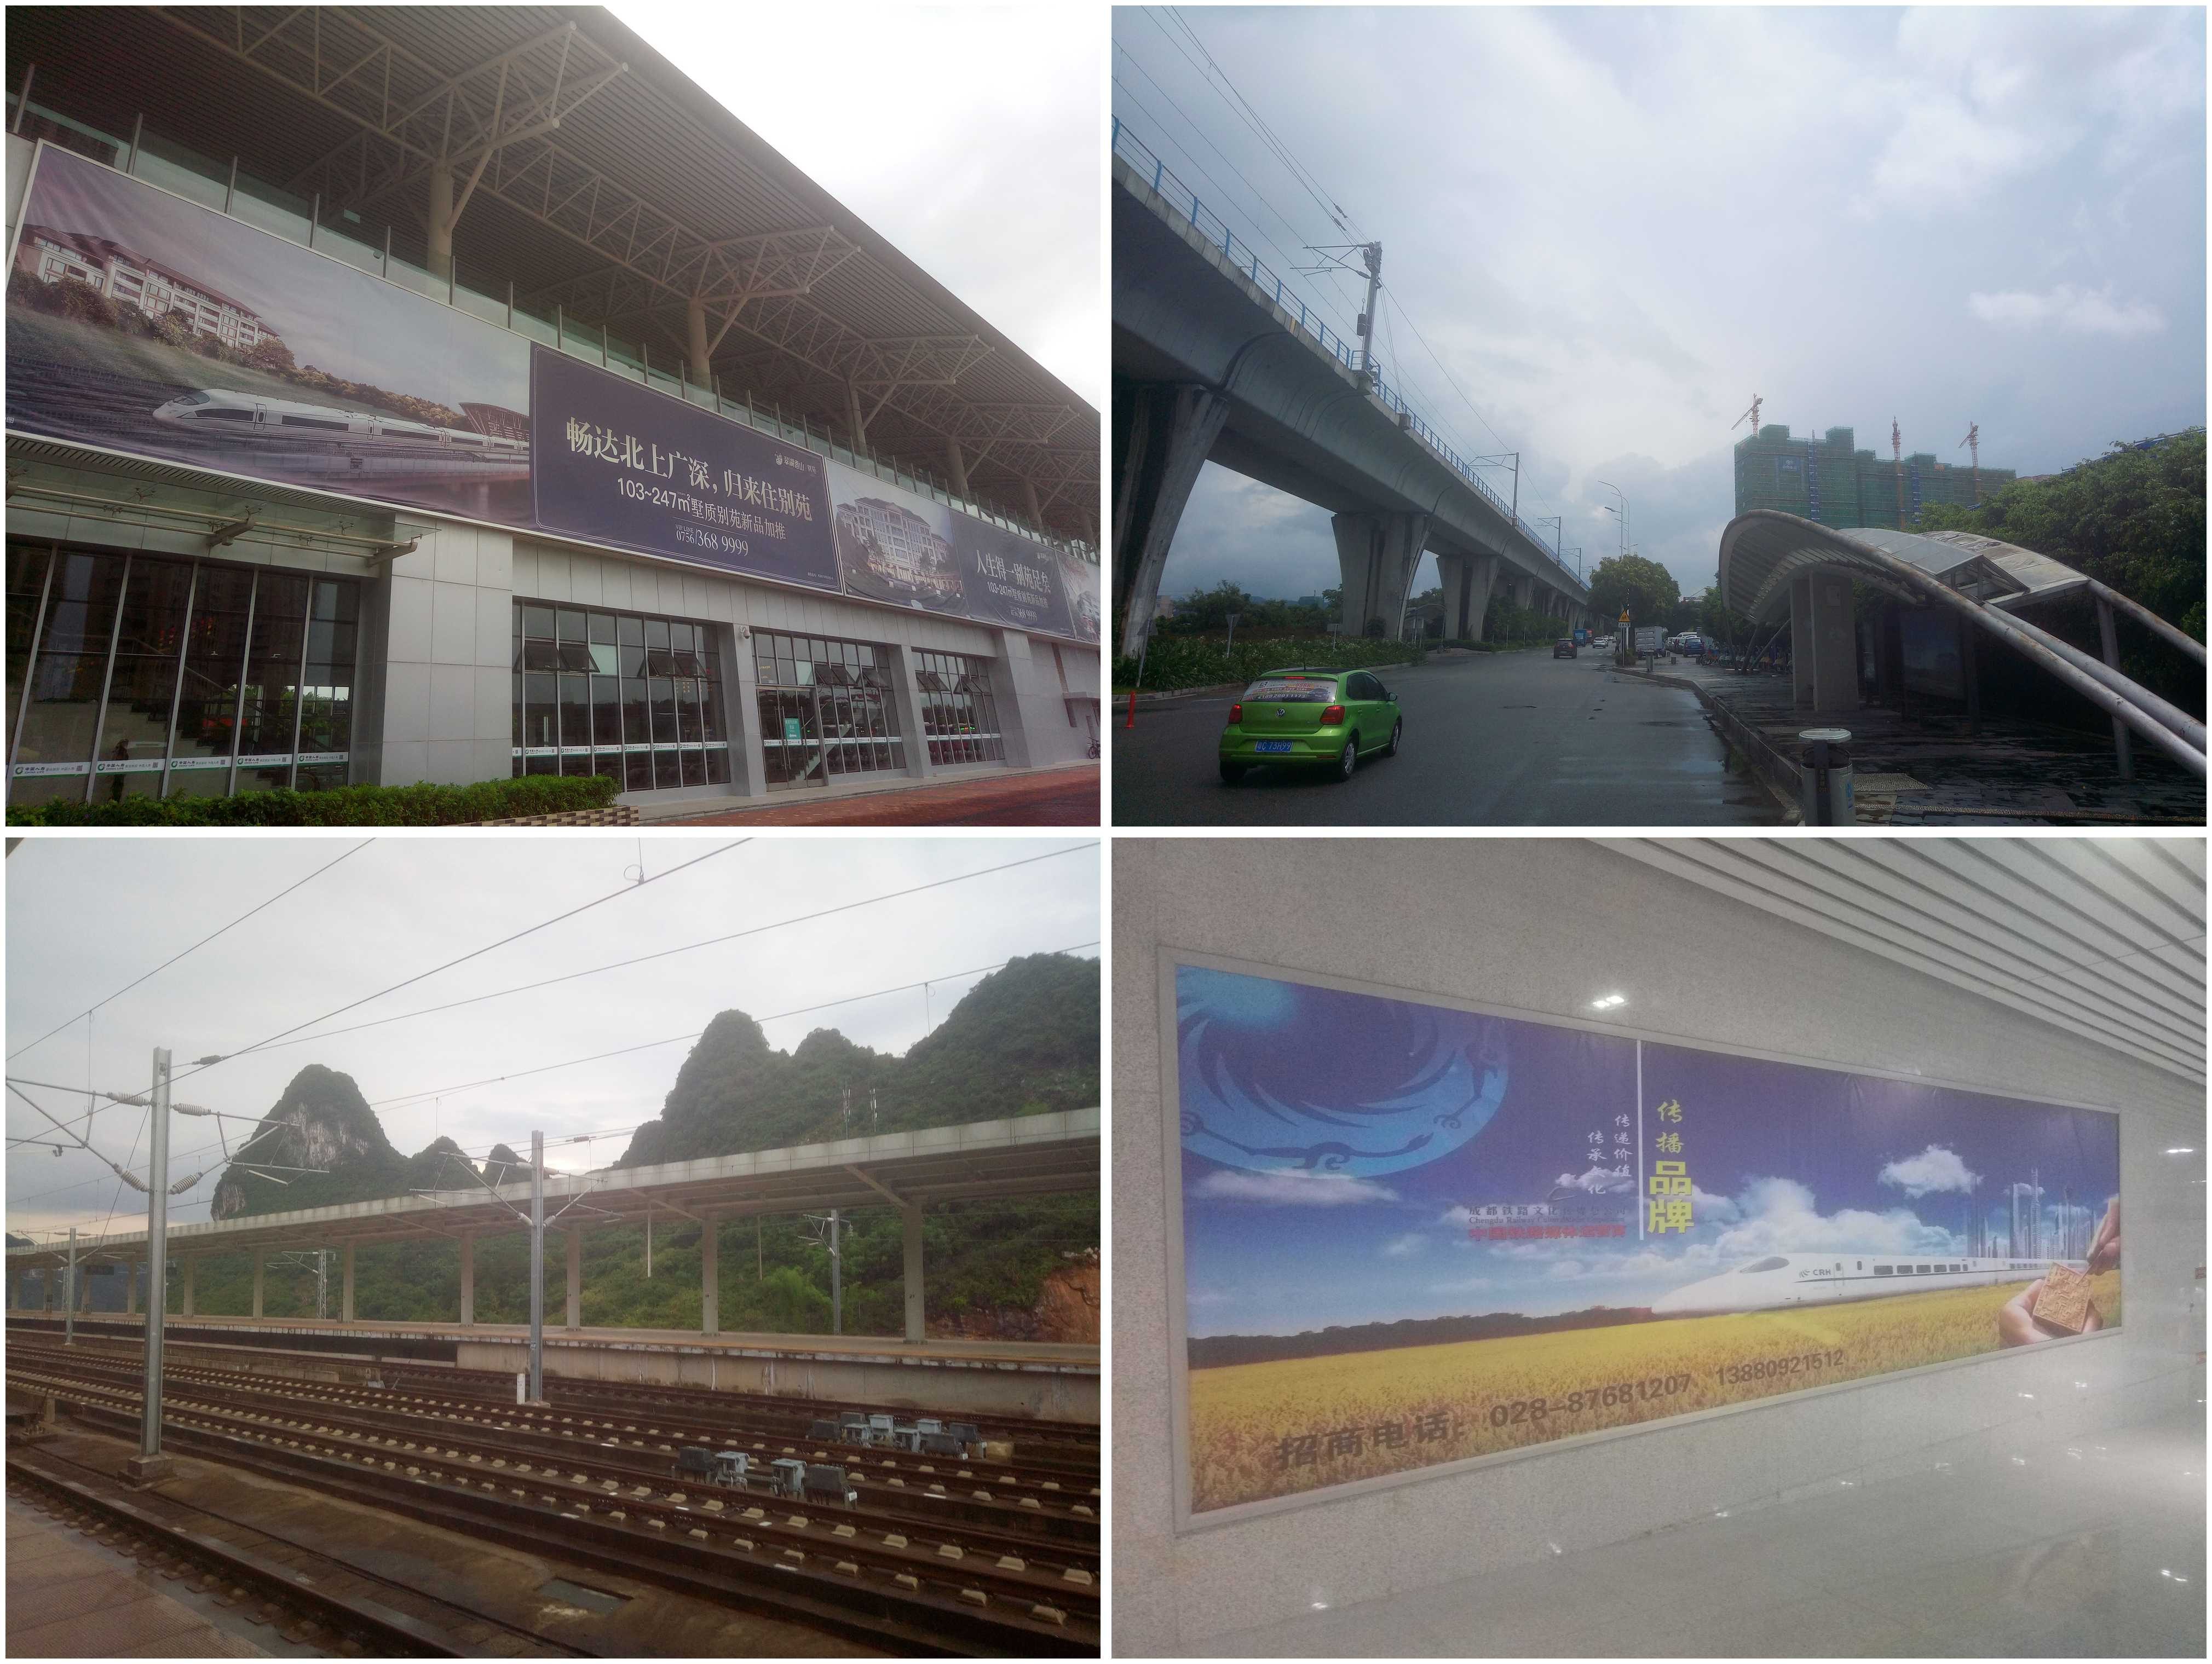
\includegraphics[width=0.9\textwidth]{figures/1-3-1-fig-qualitative-hsr.jpg}

}

\sframe{Interactions entre réseaux et territoires}{

\centering

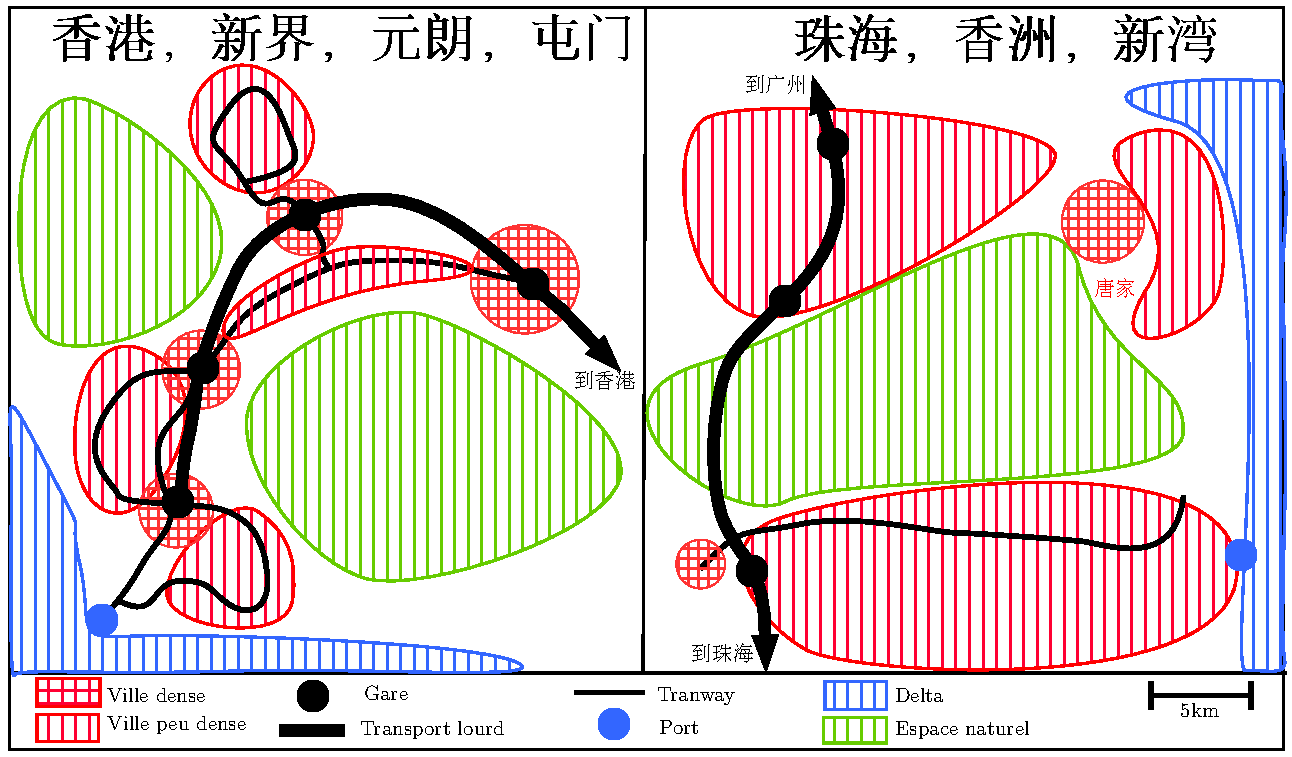
\includegraphics[width=\textwidth]{figures/1-3-1-fig-qualitative-schema.pdf}

}



\sframe{Réseaux de transport et accessibilité}{

\centering

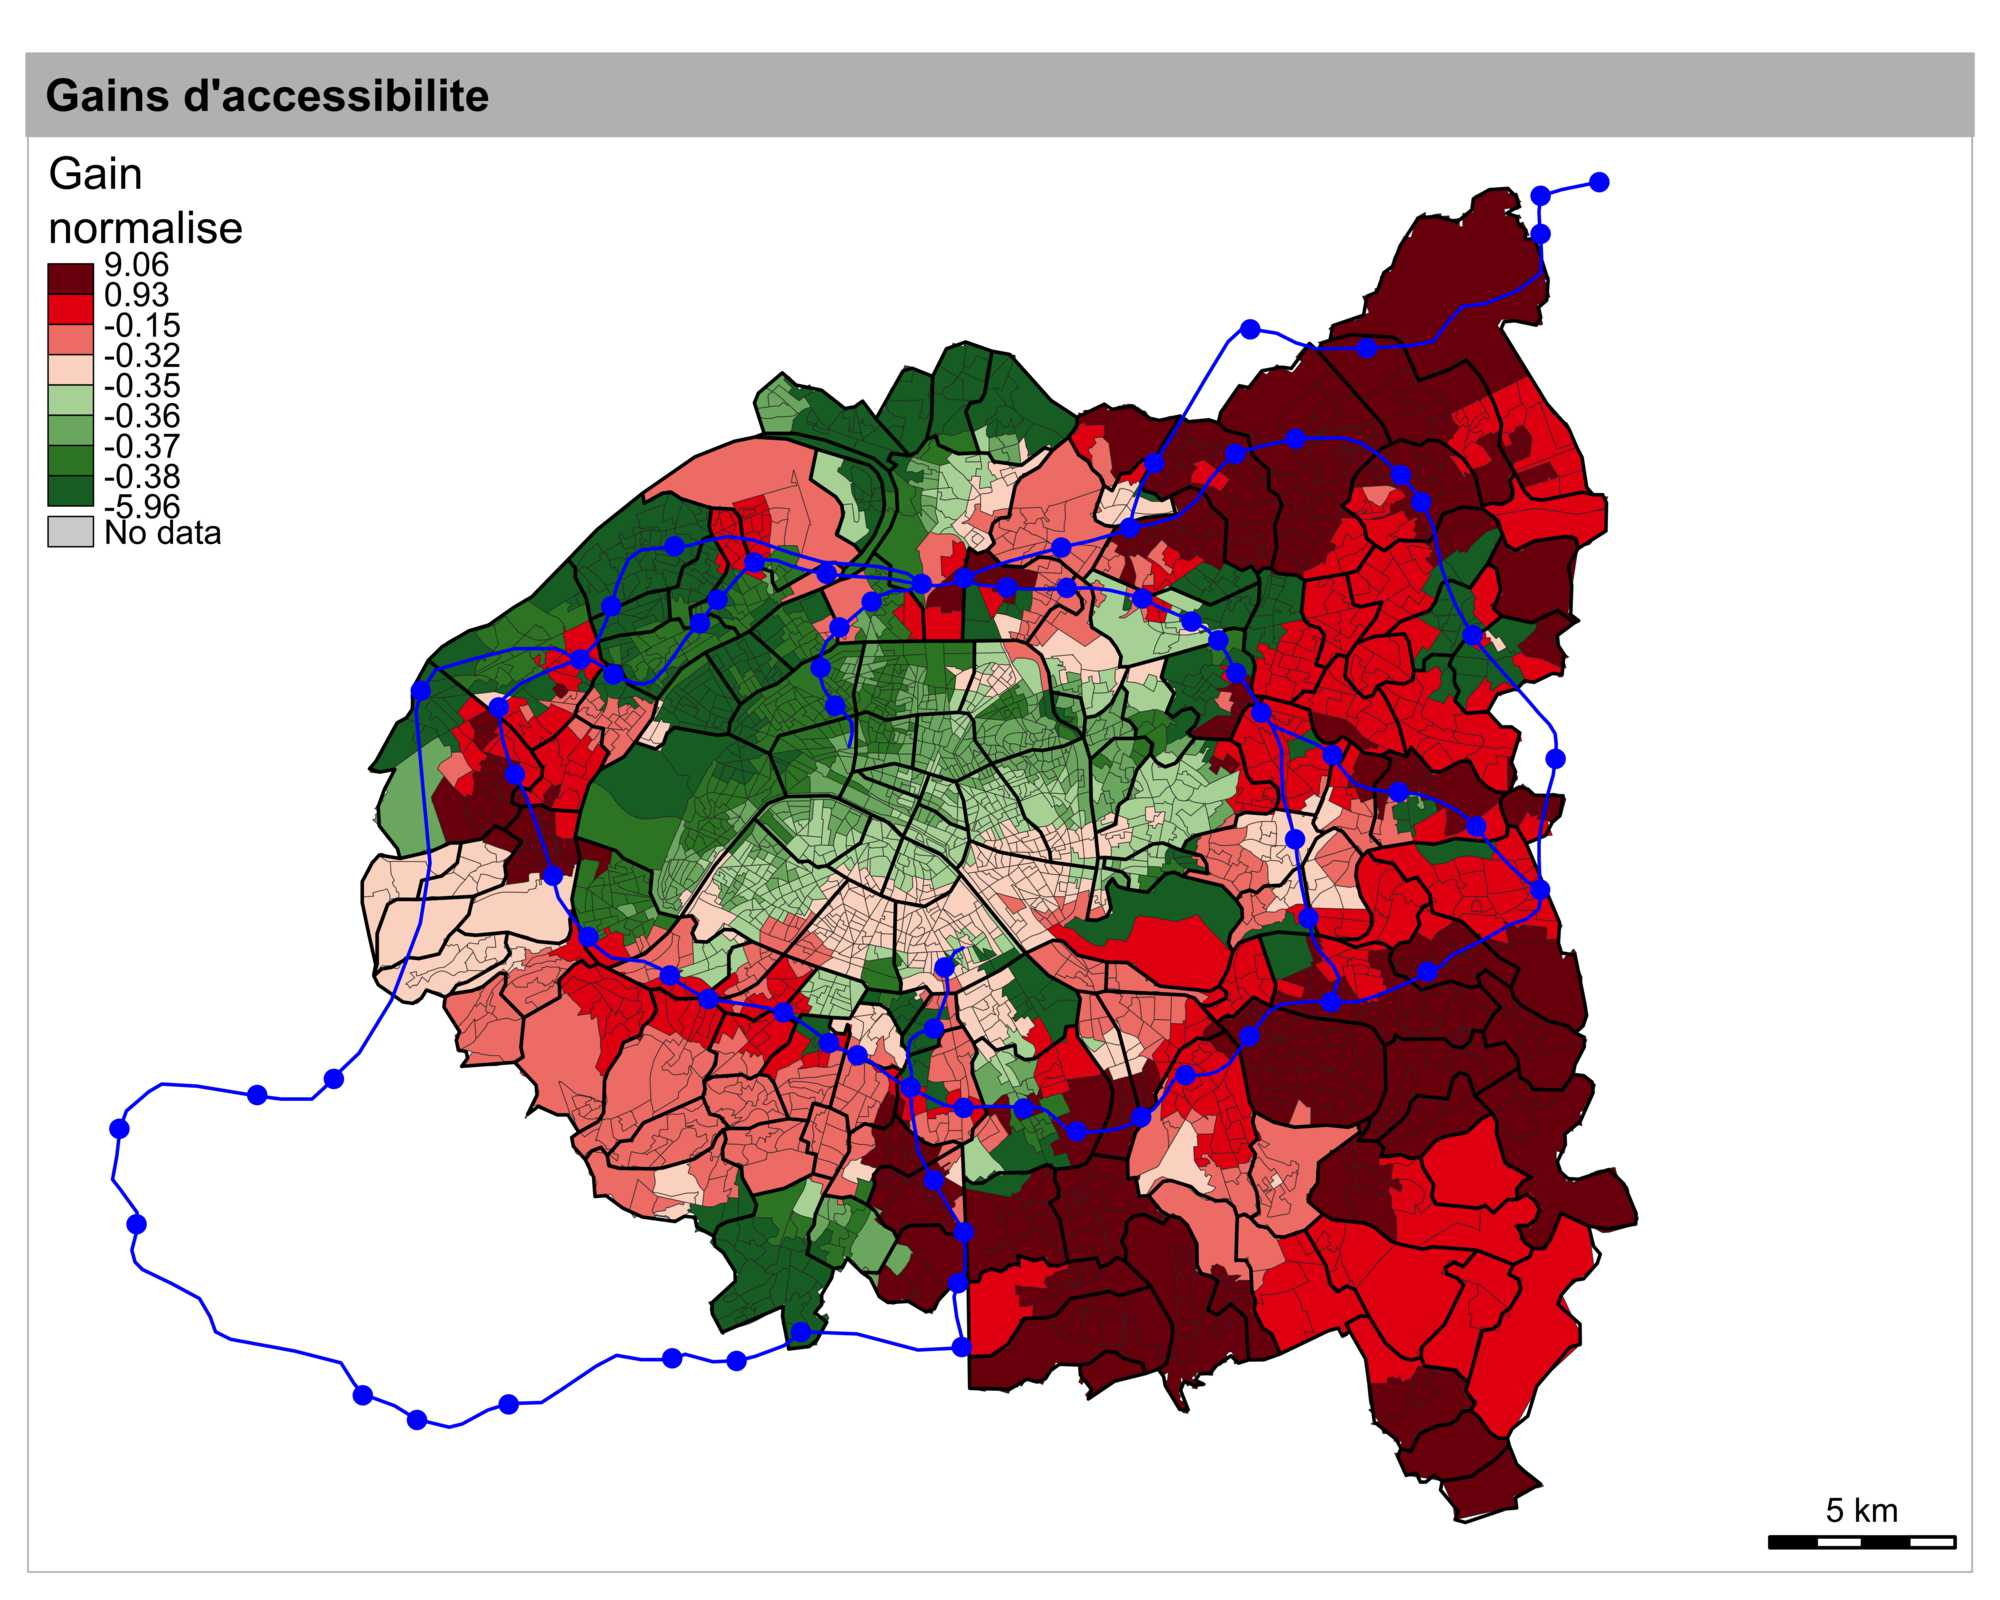
\includegraphics[width=0.9\textwidth]{figures/1-2-1-fig-casestudies-gpe.jpg}

}


\sframe{Effets structurants des réseaux}{

\centering

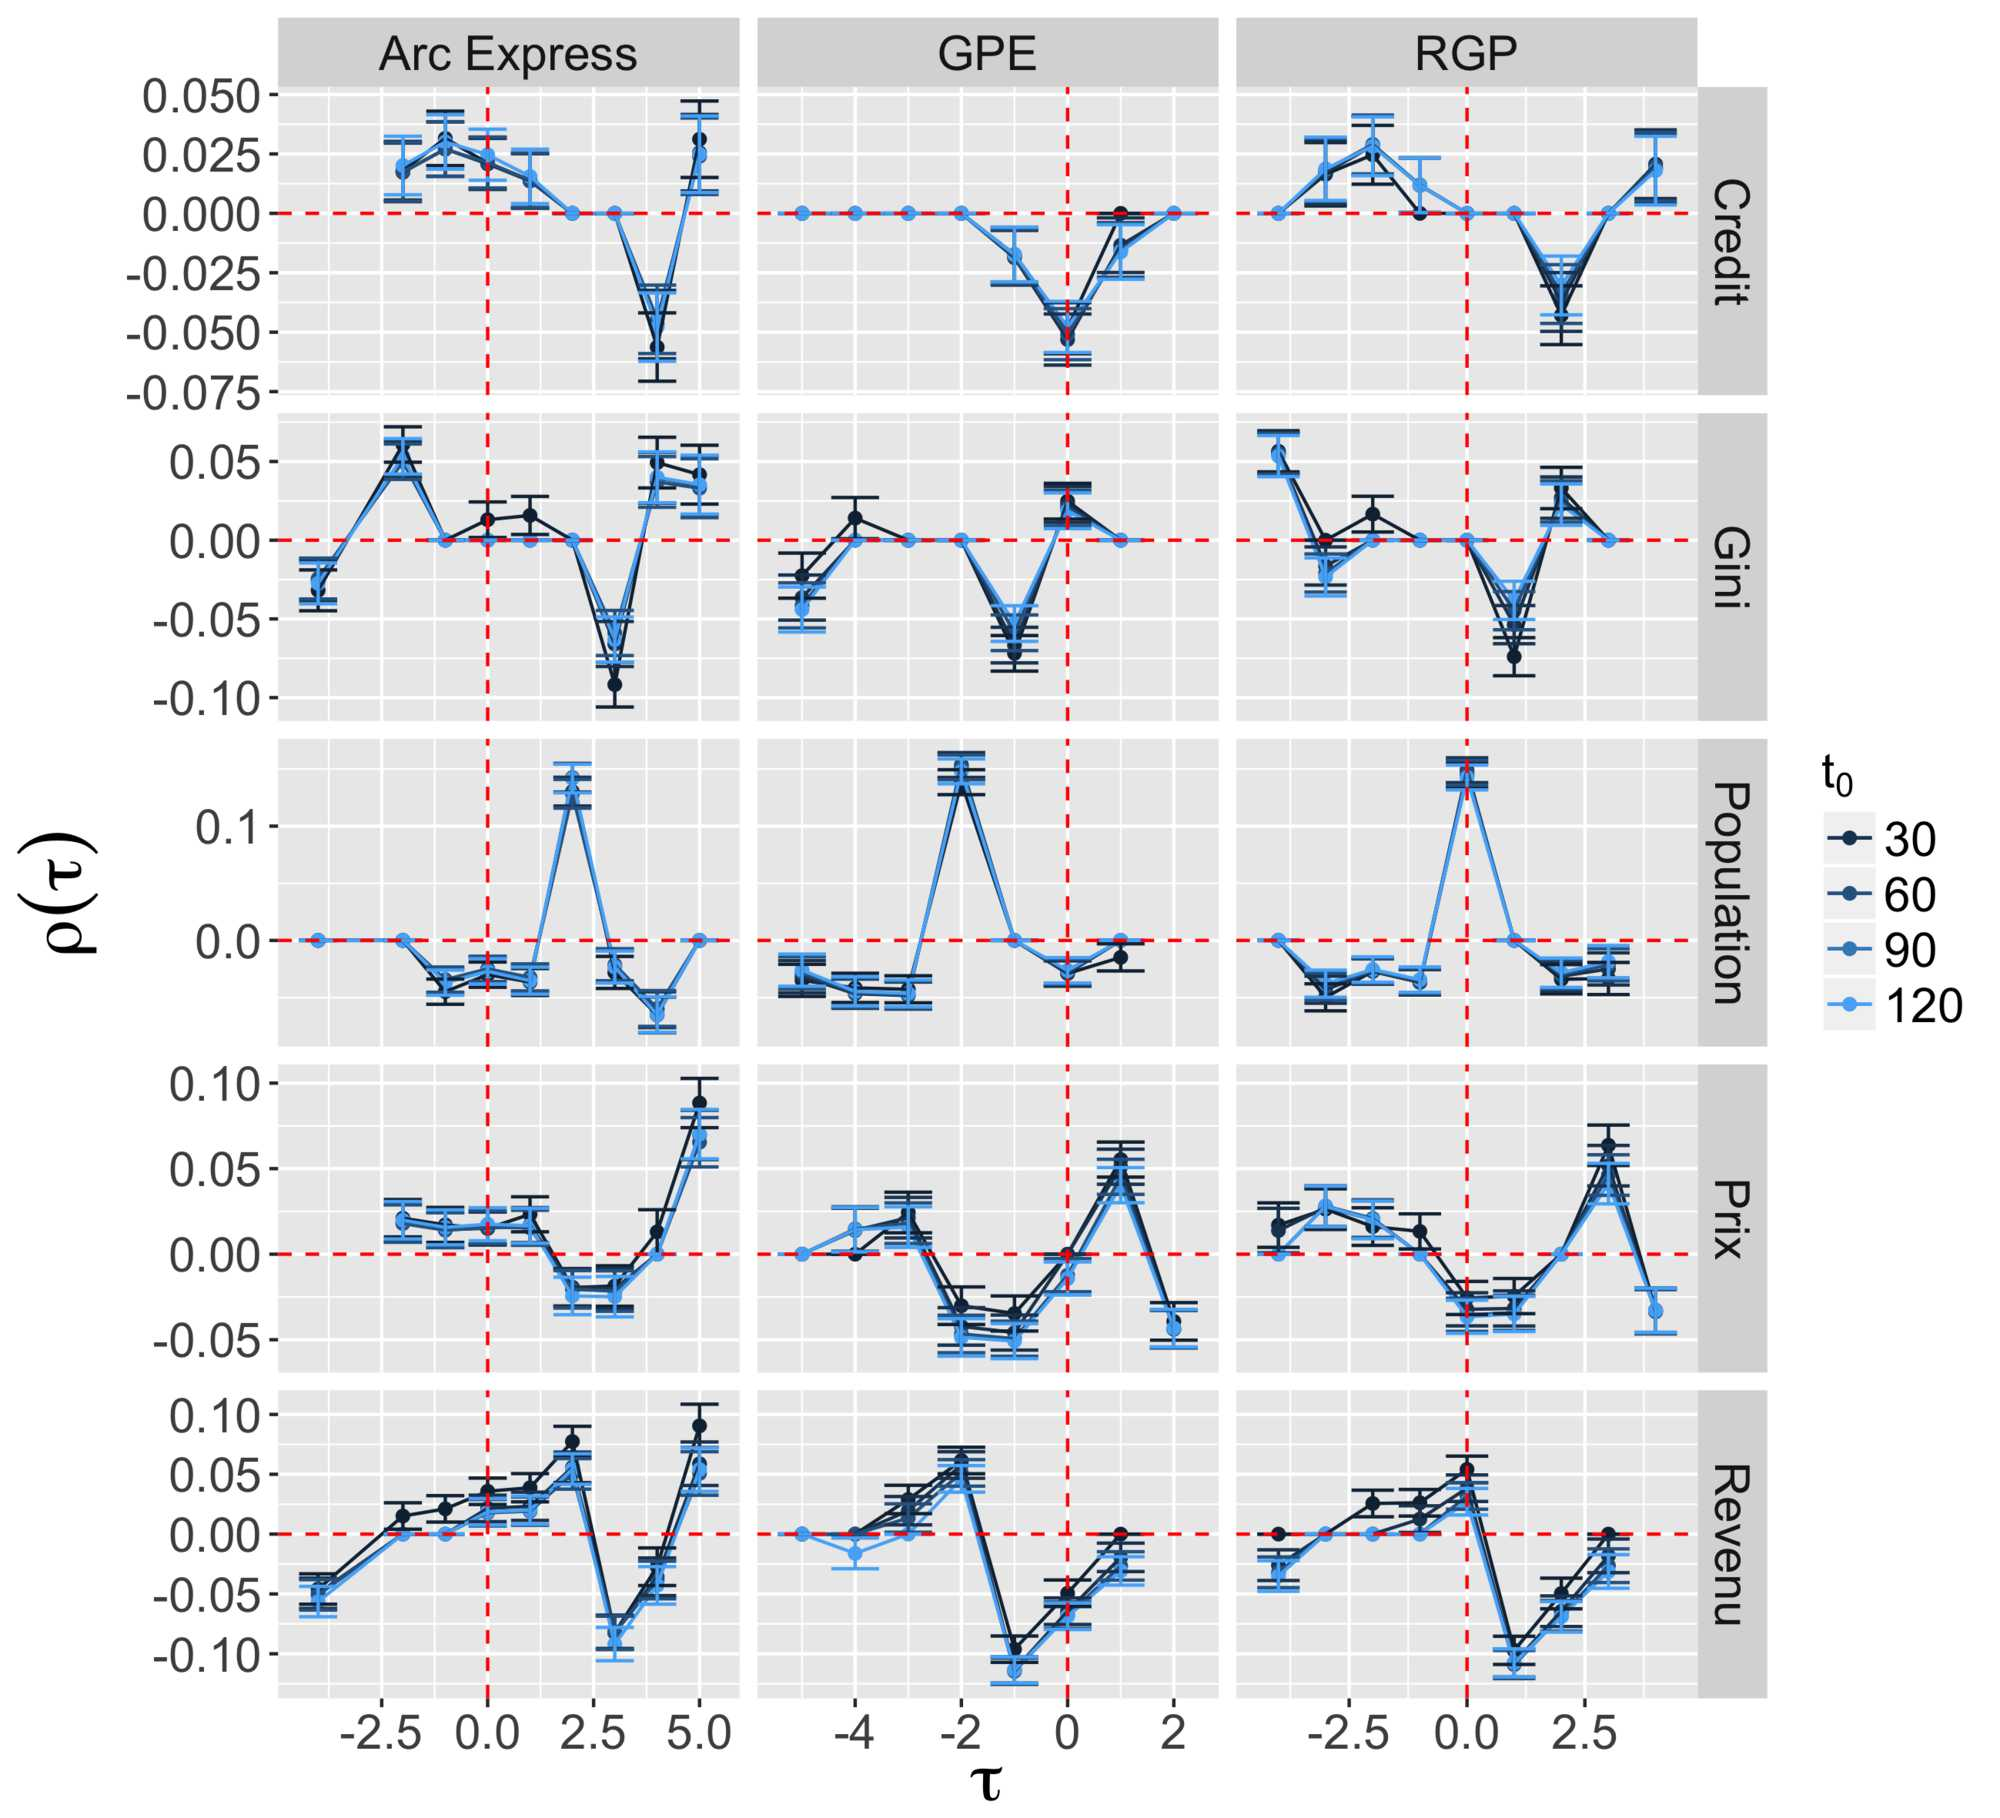
\includegraphics[width=0.8\textwidth]{figures/1-2-1-fig-casestudies-empiricalres.jpg}

}




\sframe{Modéliser réseaux et territoires}{

% paysage scientifique

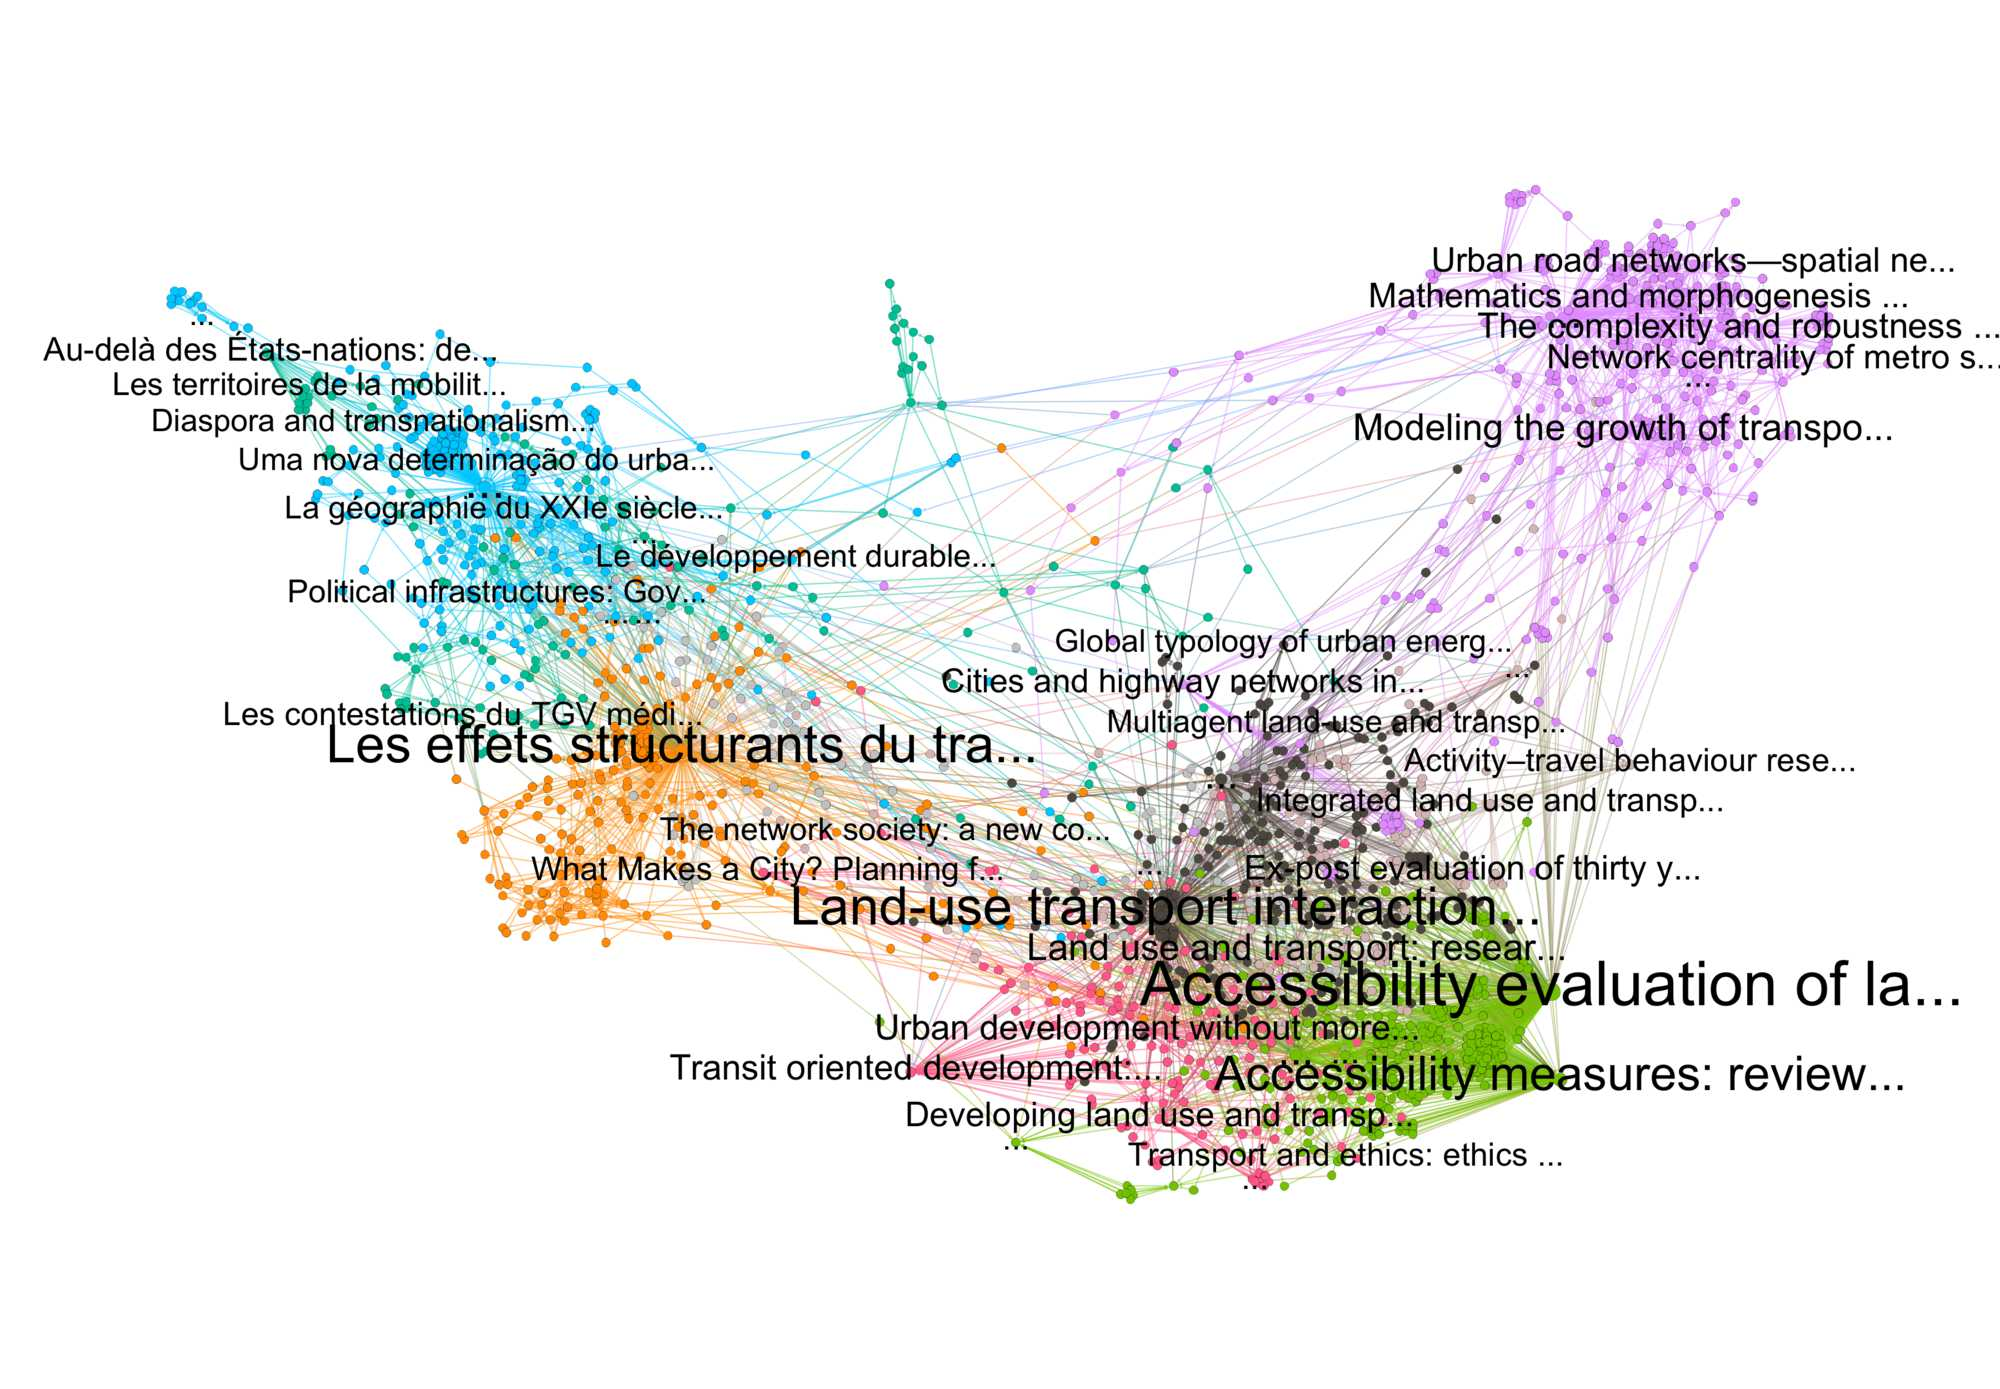
\includegraphics[width=\textwidth]{figures/2-2-2-fig-quantepistemo-citnw.jpg}

}


\sframe{Modélographie}{

\centering
% 

\footnotesize

\scalebox{.68}{
\begin{tabular}{|l|p{5cm}|p{5cm}|p{5cm}|}
\hline
 & Networks $\rightarrow$ Territories & Territories $\rightarrow$ Networks & Networks $\leftrightarrow$ Territories\\ \hline
\multirow{2}{*}{Micro} &
\textbf{Economics: } real estate market, relocalization, employment market & NA & \textbf{Computer Science : } spontaneous growth \\\cline{2-2}
& \textbf{Planning: } regulations, development & & \\\hline
& \textbf{Economics: } real estate market, transportation costs, amenities & \textbf{Economics: } network growth, offer and demand & \textbf{Economics: } investments, relocalizations, offer and demand, network planning\\\cline{2-4}
\multirow{2}{*}{Meso}& \textbf{Geography: } land-use, centrality, urban sprawl, network effects & \textbf{Transportation: } investments, level of governance & \textbf{Geography: } land-use, network growth, population diffusion \\\cline{2-3}
& \textbf{Planning/transportation: } accessibility, land-use, relocalization, real estate market & \textbf{Physics: } topological correlations, hierarchy, congestion, local optimization, network maintenance & \\\hline
& \textbf{Economics: } economic growth, market, land-use, agglomeration, sprawl, competition & \textbf{Economics: } interactions between cities, investments & \textbf{Economics: } offer and demand \\ \cline{2-4}
\multirow{2}{*}{Macro} & \textbf{Geography: } accessibility, interaction between cities, relocalization, political history & \textbf{Geography: } interactions between cities, potential breakdown & \textbf{Transportation: } network coverage \\\cline{2-3}
& \textbf{Transportation: } accessibility, real estate market & \textbf{Transportation: } network planing & \\\hline
\end{tabular}
}

}

\sframe{Modèles LUTI}{

% cadre theorique : Wegener

Cadre théorique pour les modèles \textit{Land-use transport interaction} \cite{wegener2004land}

\medskip

\centering

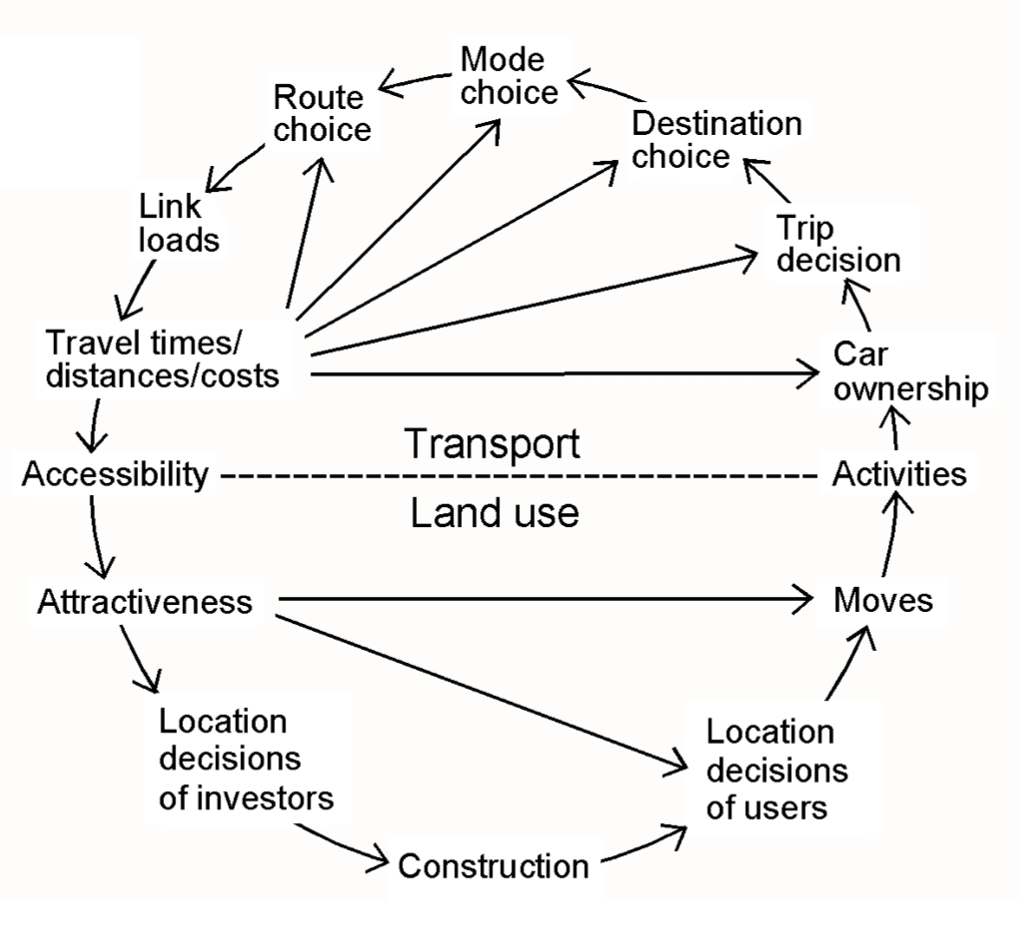
\includegraphics[height=0.8\textheight]{figures/luti_framework.png}

}


\sframe{Complexification des LUTI \cite{wegener2004land}}{
\centering
   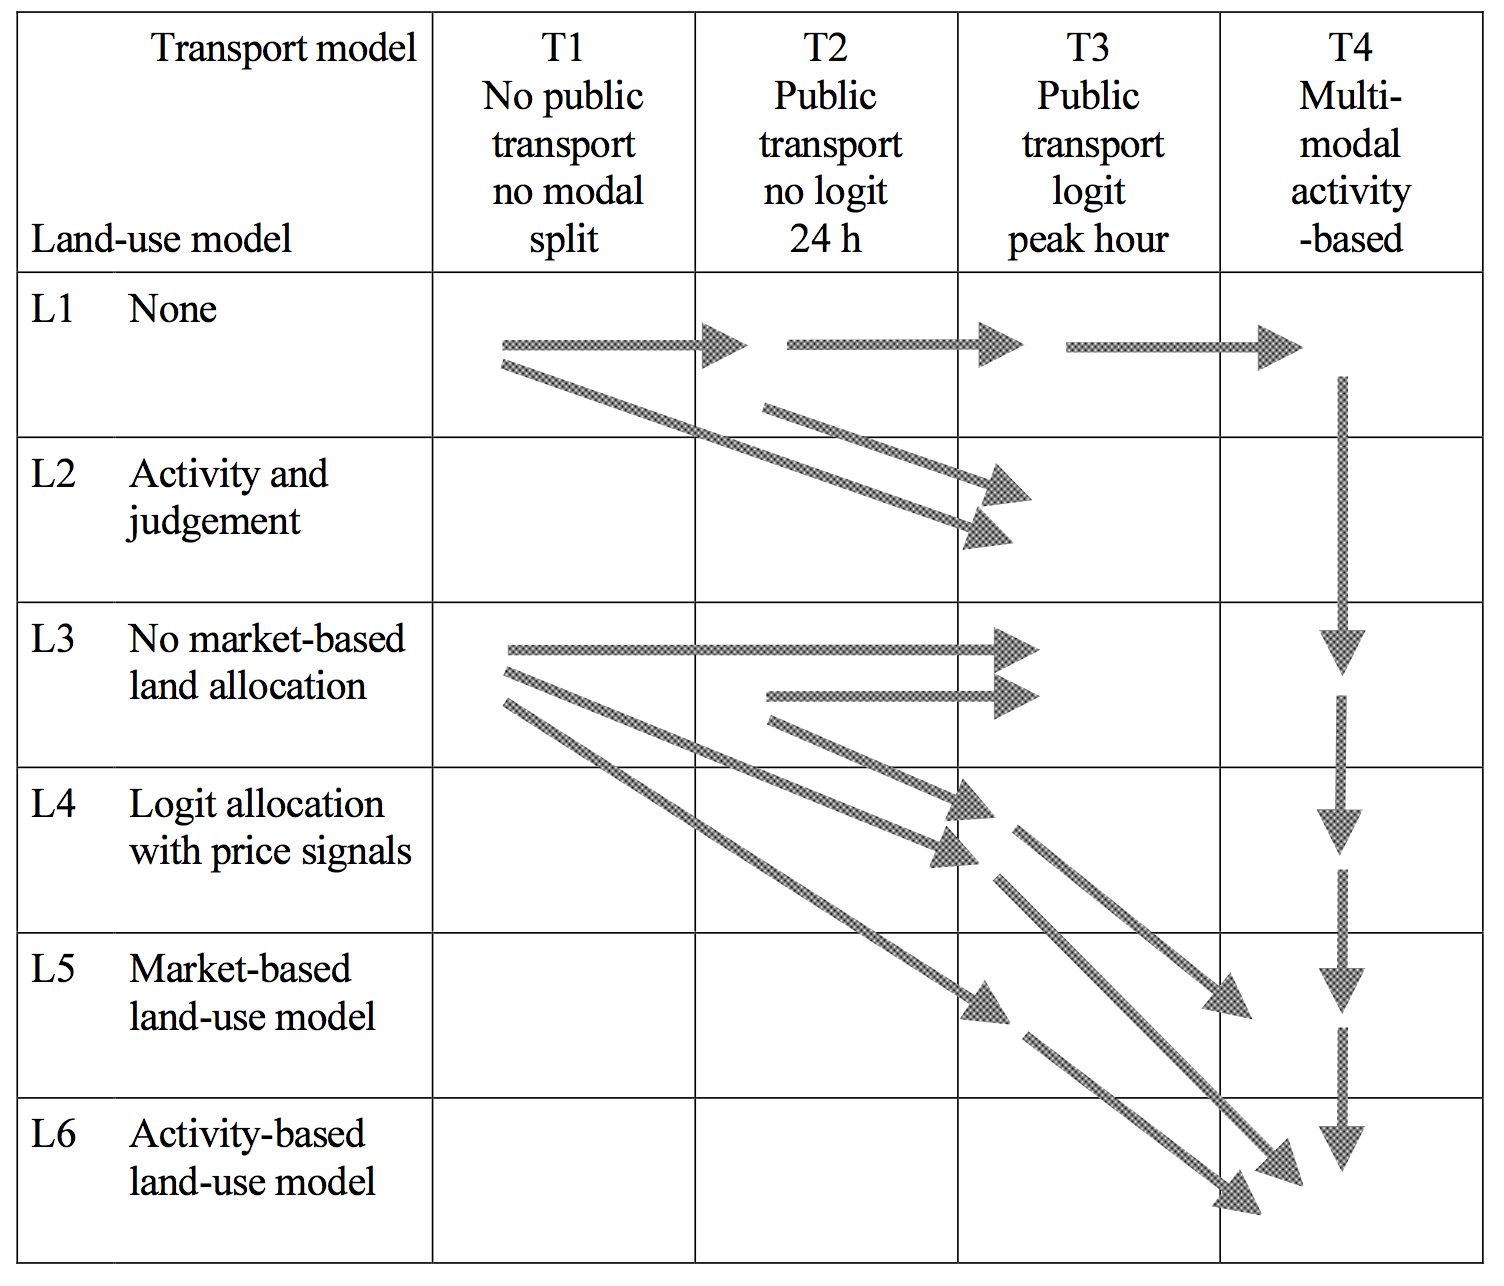
\includegraphics[height=0.86\textheight]{figures/luti_complexity.png}
}

\sframe{Processus dans des LUTI \cite{wegener2004land}}{

	\centering

  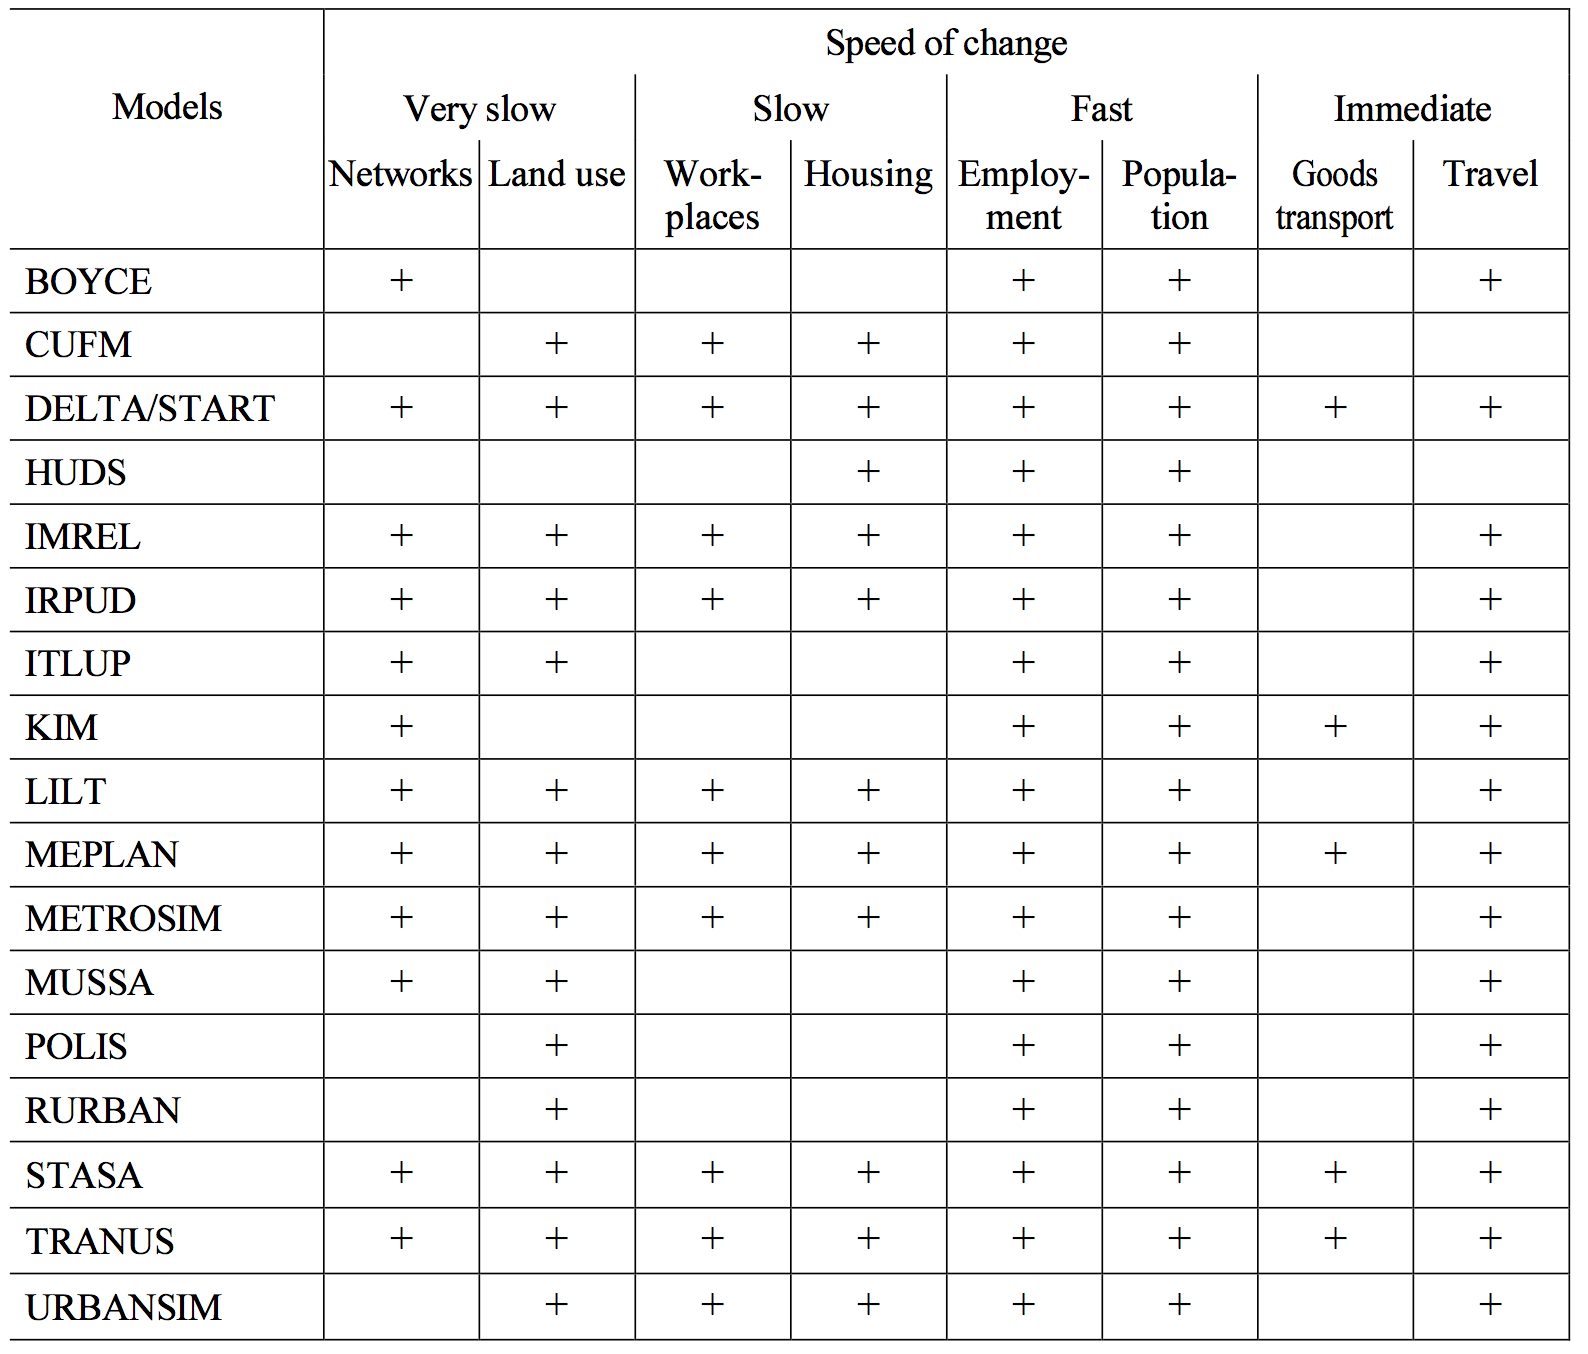
\includegraphics[height=0.9\textheight]{figures/luti_models.png}
}

\sframe{Un exemple: le modèle Nedum}{

\textit{Interaction entre prix immobiliers, coût de transport et densité de population} \cite{viguie2014downscaling}

\medskip

\centering

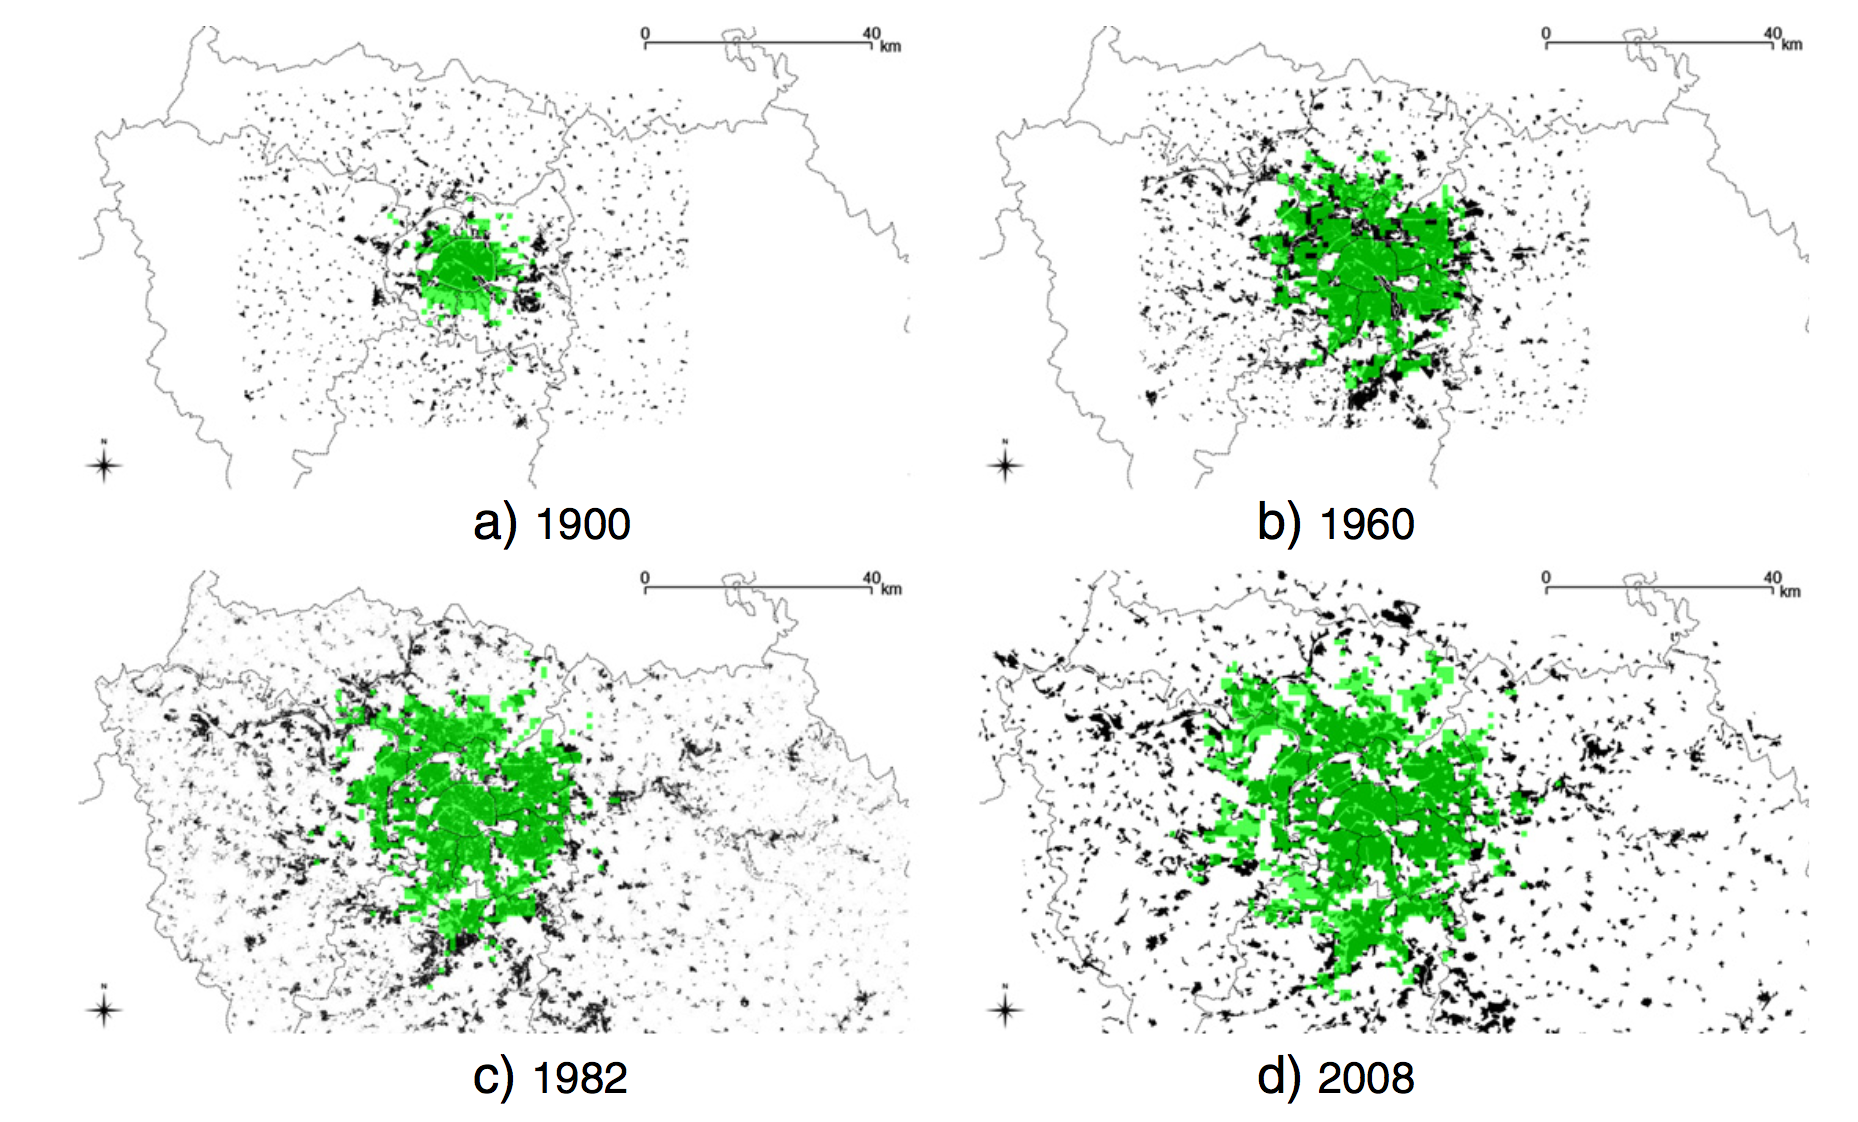
\includegraphics[width=0.95\textwidth]{figures/nedum_example.png}

}

\sframe{Modèle stylisé pour le test des méthodes}{

\textit{Relocalisations actifs/emplois basées sur un compromis entre accessibilité et densité, réseau de transport dynamique sur le temps long} \cite{le2015modeling}

\medskip
\centering

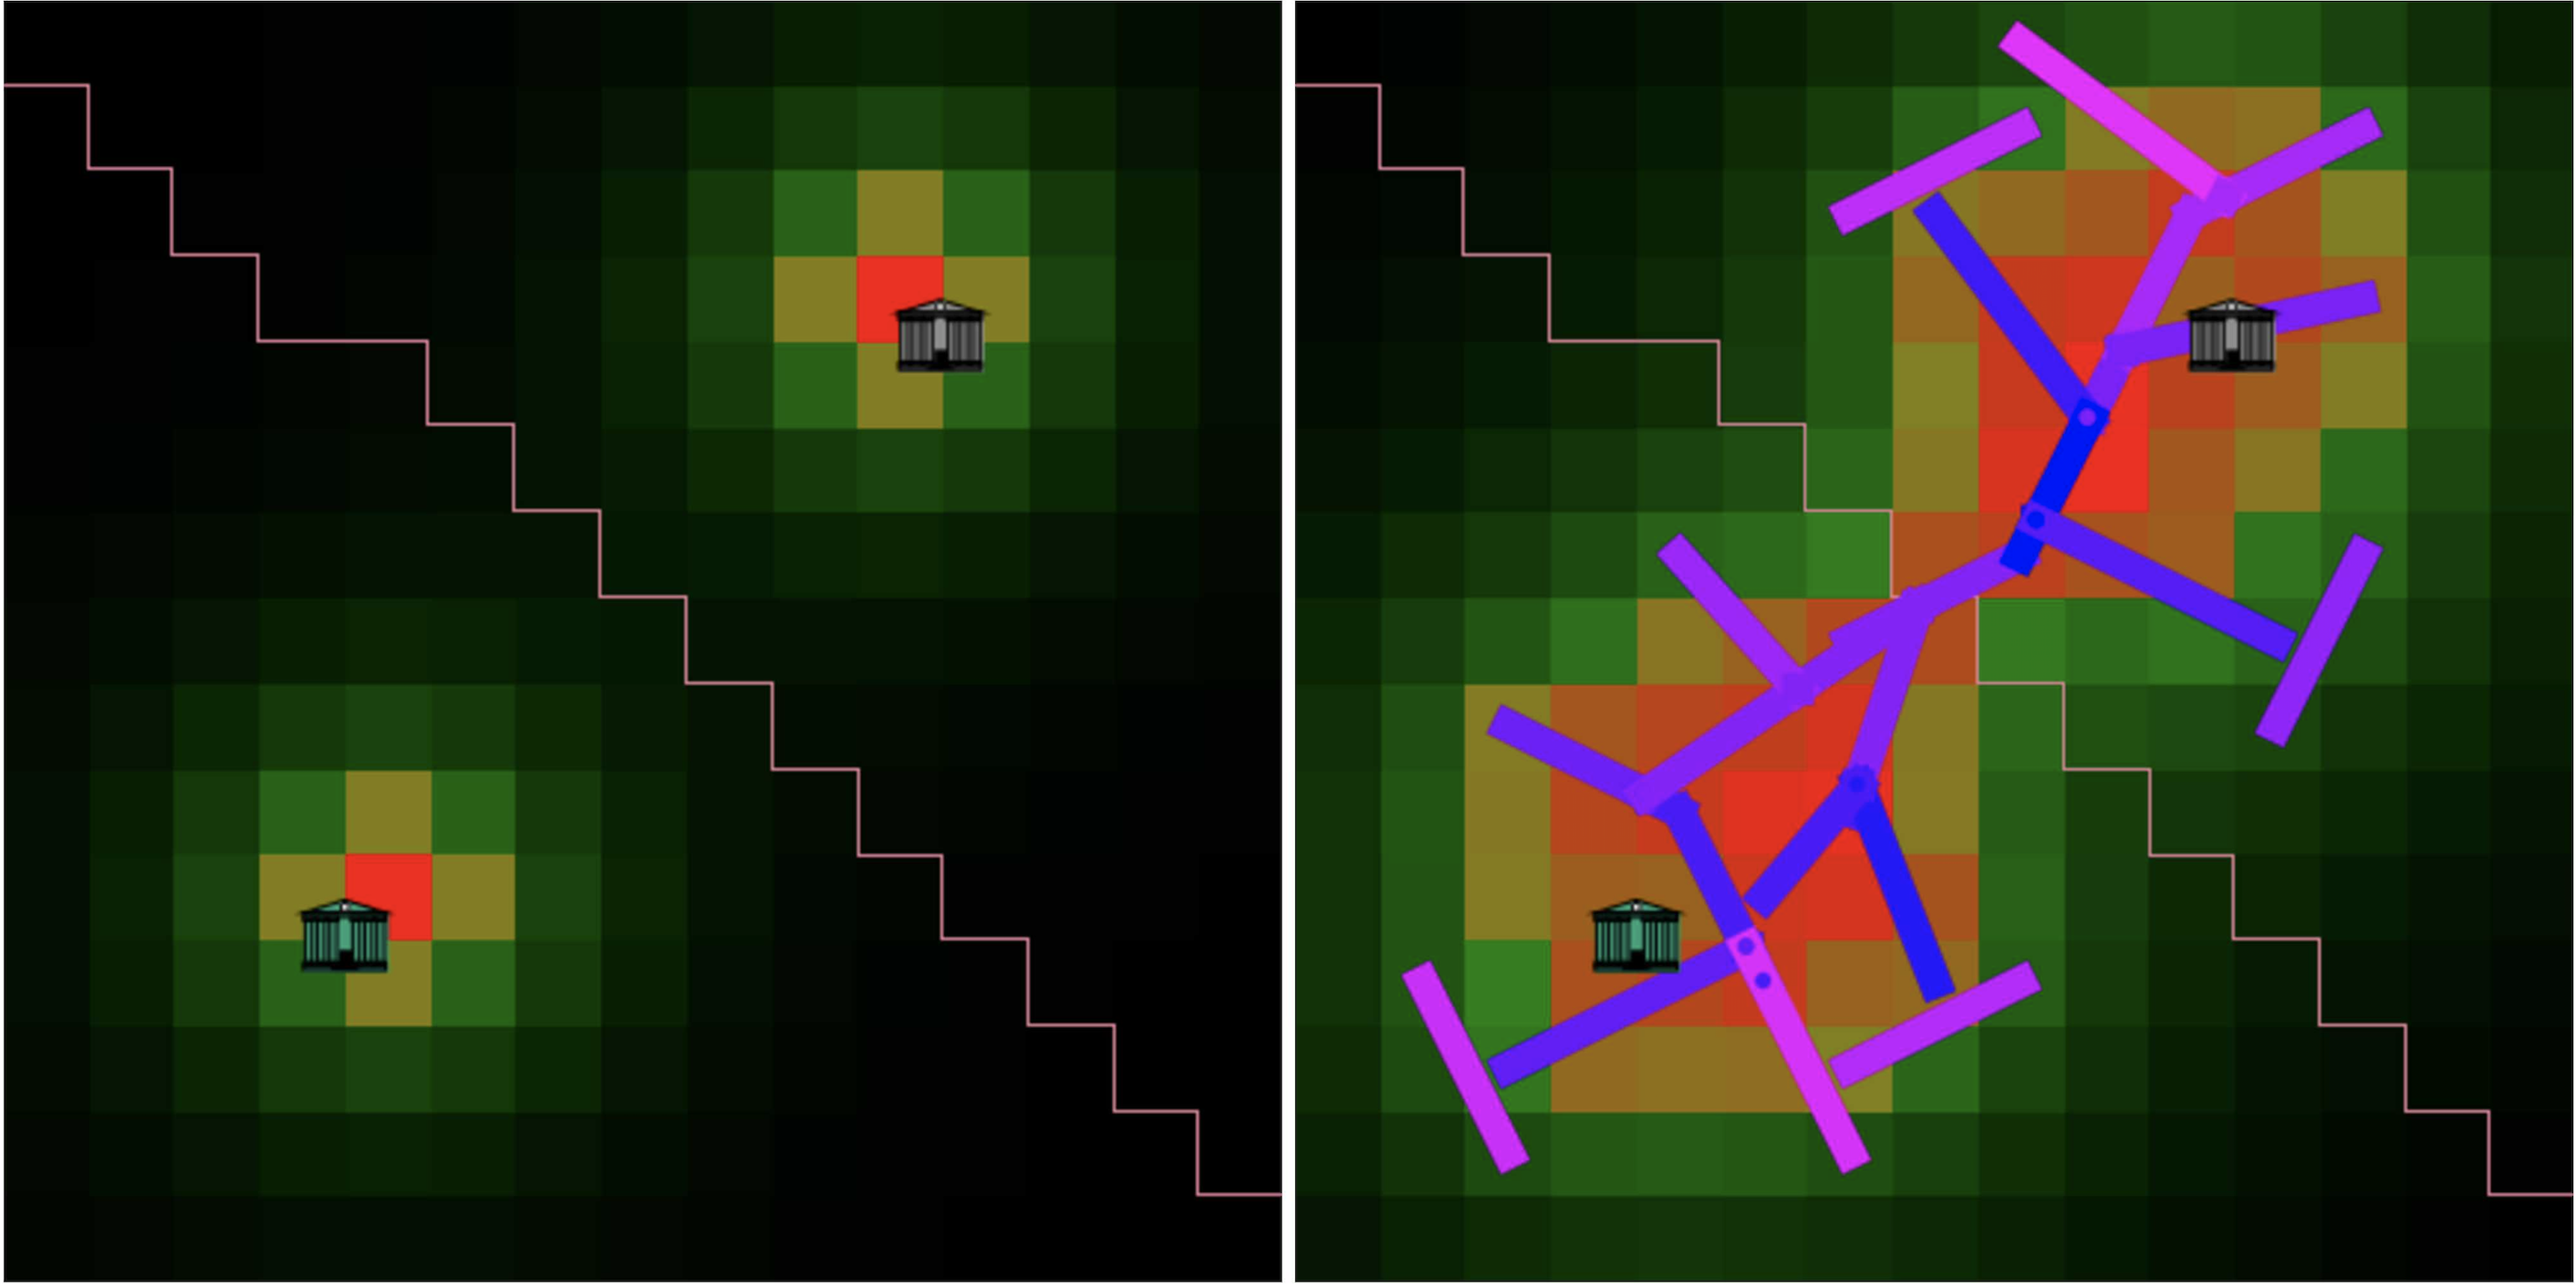
\includegraphics[width=0.95\textwidth]{figures/meso-lutecia.jpg}

}

\sframe{Modèle Dynamicity}{

\textit{Basé sur le modèle UrbanSim, principalement modèle de choix discrets pour la (re-)localisation des actifs}

\medskip

\begin{itemize}
	\item Offre d'emplois et réseaux de transport (multimodal) exogènes
	\item Structure de population synthétique générée par un modèle amont
	\item Croissance de la population à l'échelle de l'agglomération simulée générée par un modèle amont
	\item Localisation des nouveaux arrivants, successives, suivant un modèle de choix discrets, estimé sur la première année (par segments de population)
\end{itemize}

}

\sframe{Vers des méthodes de validation}{

\textit{Pistes explorées}

\medskip

\begin{itemize}
	\item Génération de réseaux stylisés (scenarios de transport)
	\item Sensibilité et optimisation
	\item Faits stylisés à vérifier
	\item Diversité
\end{itemize}

}

\sframe{Modèle slime-mould pour générer des réseaux}{
  
  {\color{white}
          %\centering
          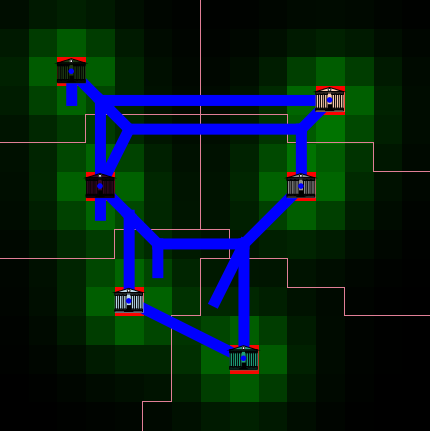
\includegraphics[width=0.33\columnwidth]{figures/bionw_territ6_gamma1_1_bis.png}\vrule width 1pt
          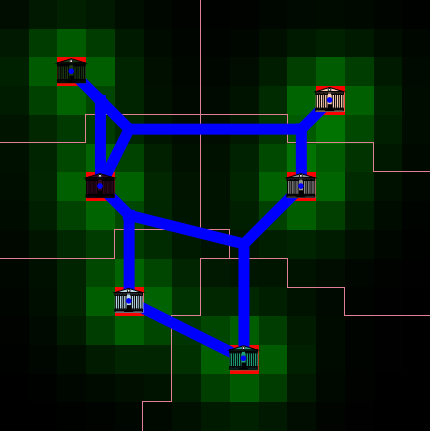
\includegraphics[width=0.33\columnwidth]{figures/bionw_territ6_gamma1_2_quart.png}\vrule width 1pt
          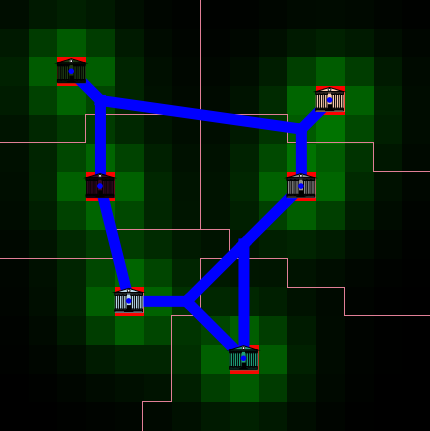
\includegraphics[width=0.33\columnwidth]{figures/bionw_territ6_gamma1_25_bis.png}\\\hrule height 1pt
          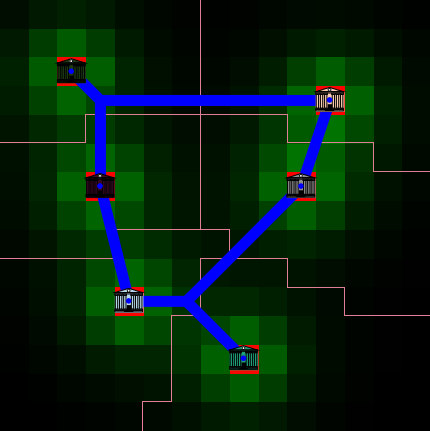
\includegraphics[width=0.33\columnwidth]{figures/bionw_territ6_gamma1_3_bis.png}\vrule width 1pt
          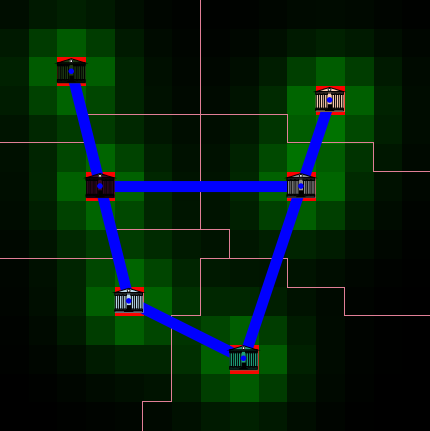
\includegraphics[width=0.33\columnwidth]{figures/bionw_territ6_gamma1_5.png}\vrule width 1pt
          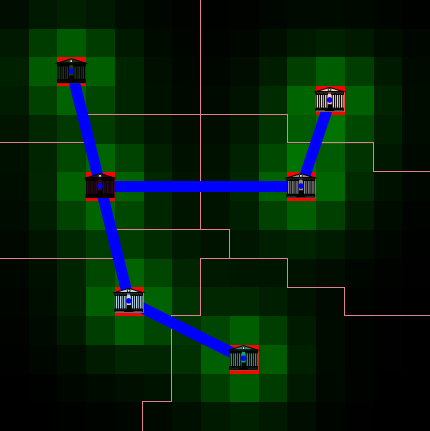
\includegraphics[width=0.33\columnwidth]{figures/bionw_territ6_gamma1_8.png}\\
          %\bigskip
          \color{black}
          
          \cite{raimbault2018systemes}
          %\small\textit{Réseaux stylisés obtenus pour des valeurs décroissantes de $\gamma$, pour une même configuration des centres de population à desservir (densité de population générée par mélange d'exponentielles).}
          }
  
}

\sframe{Optimalité des réseaux générés}{
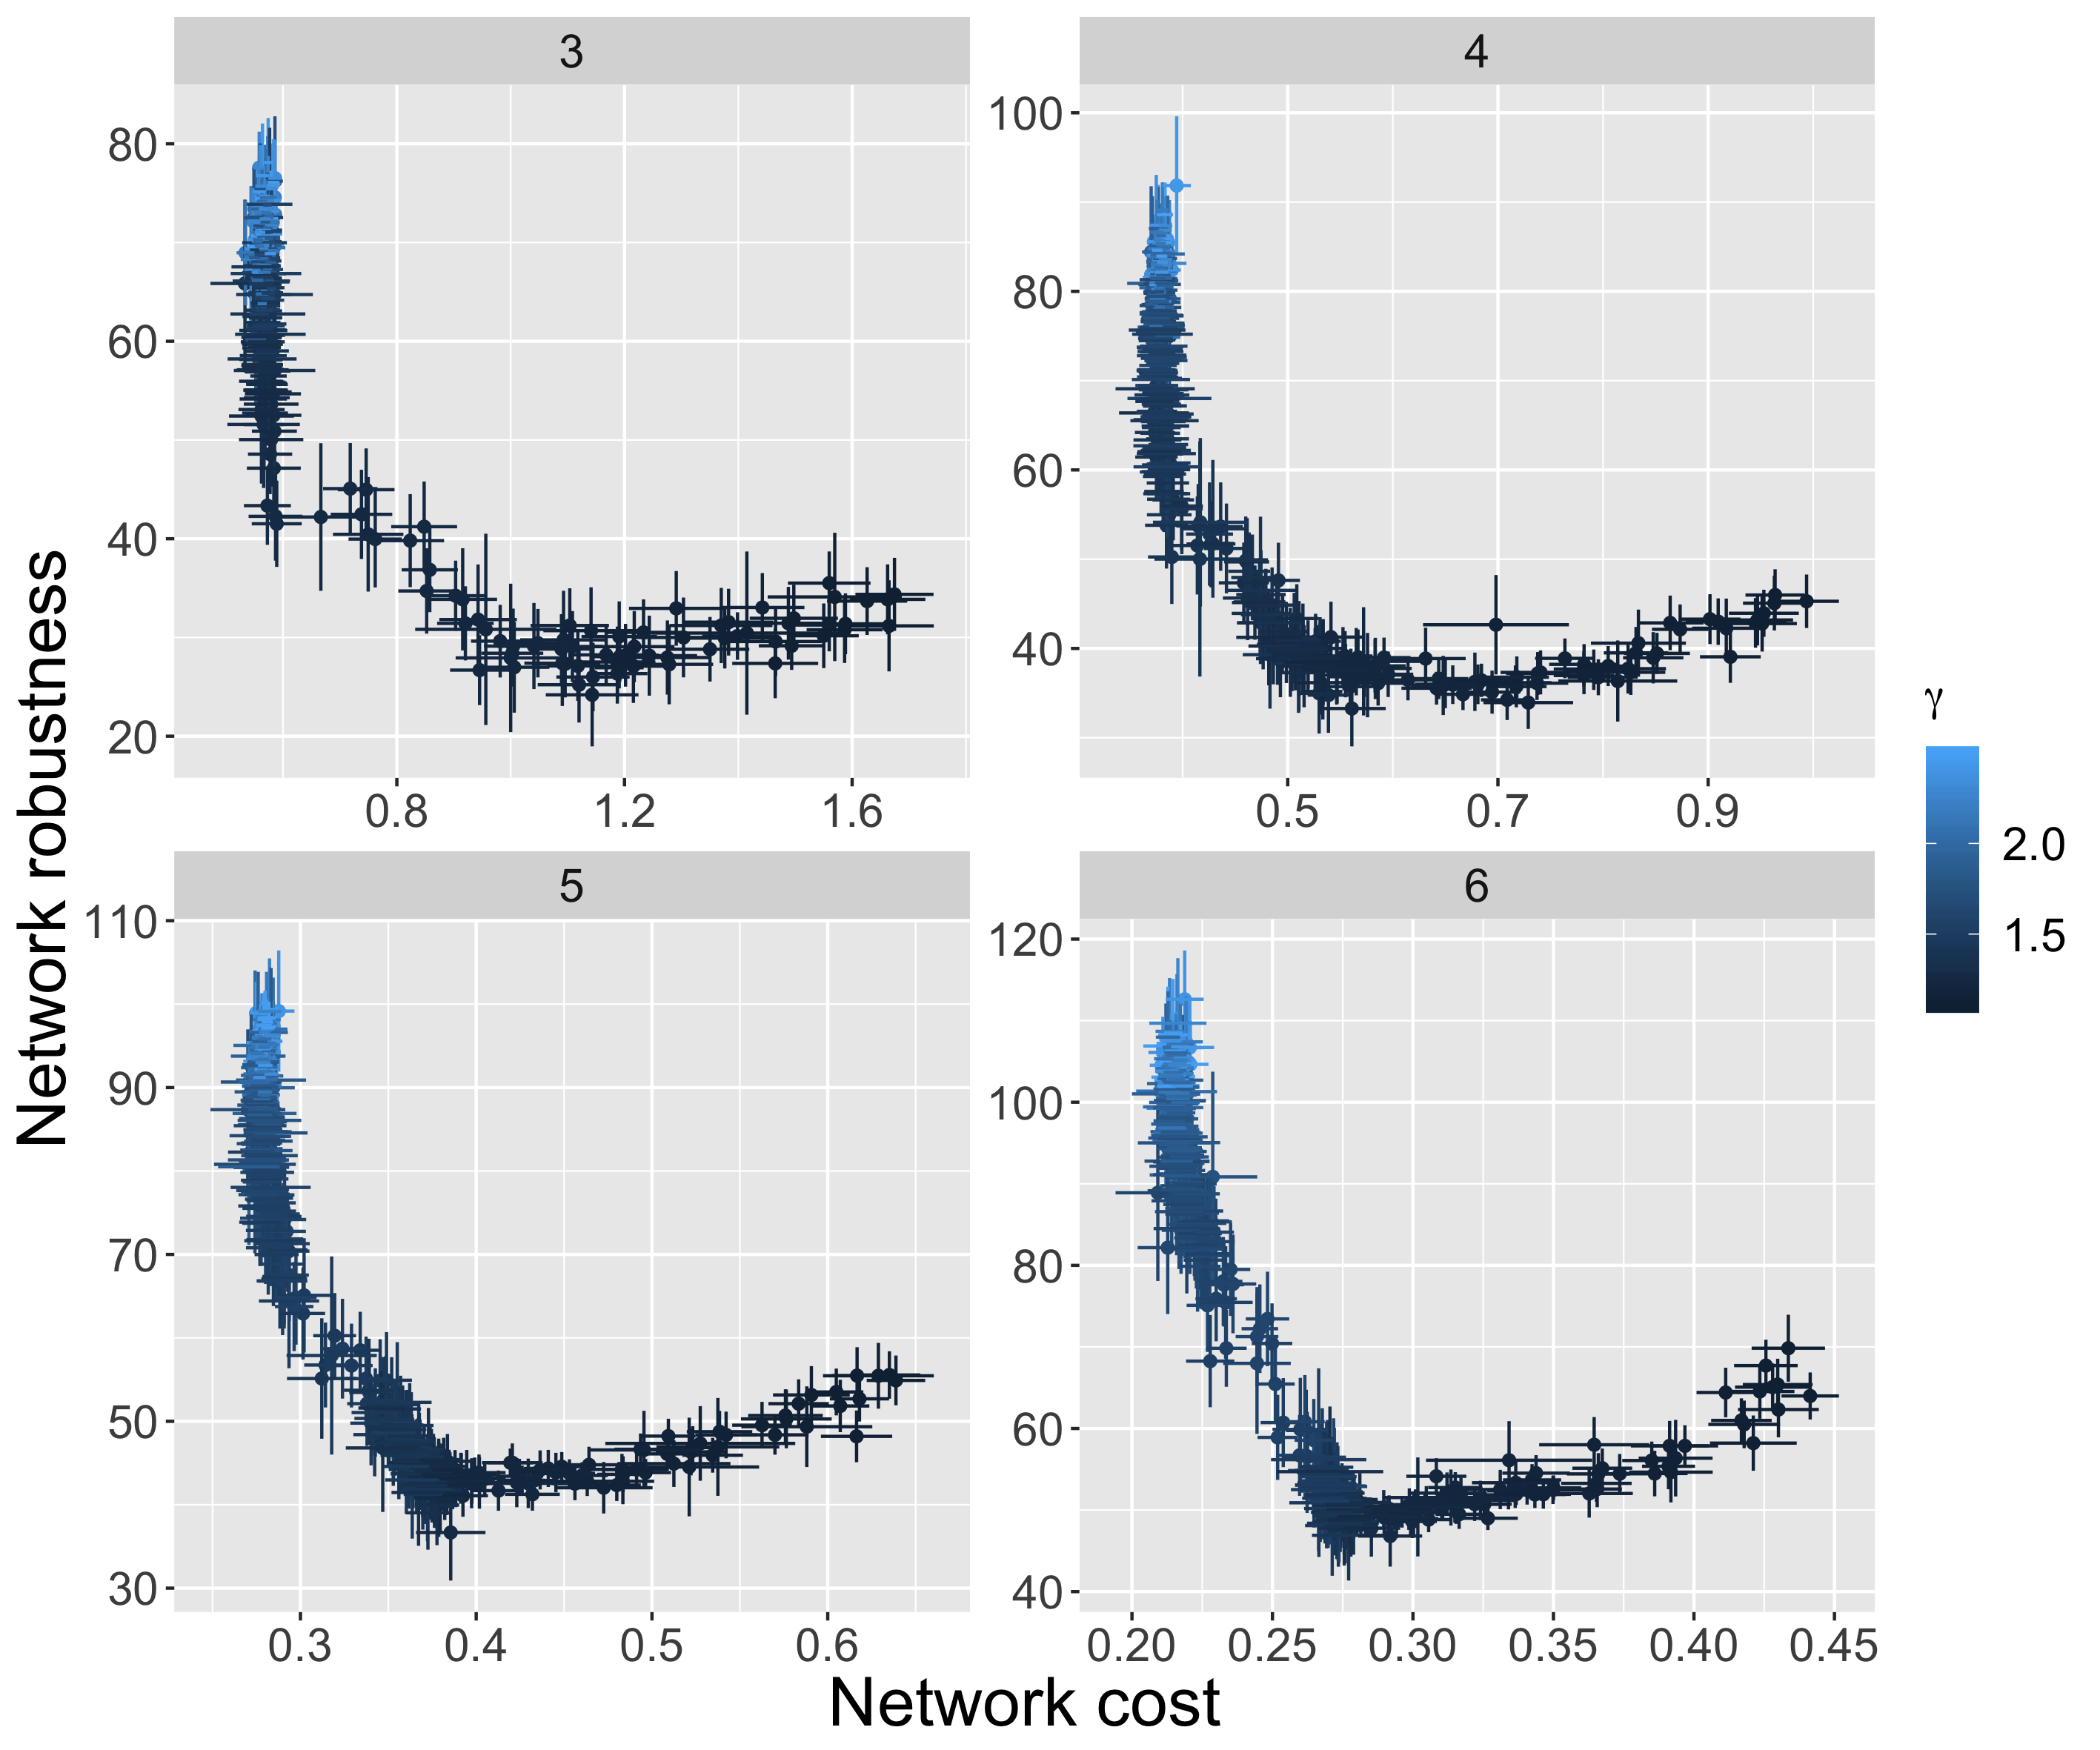
\includegraphics[width=0.5\textwidth]{figures/pareto_cost-robustness_facetCenterNumber_withgaussianCI.png}
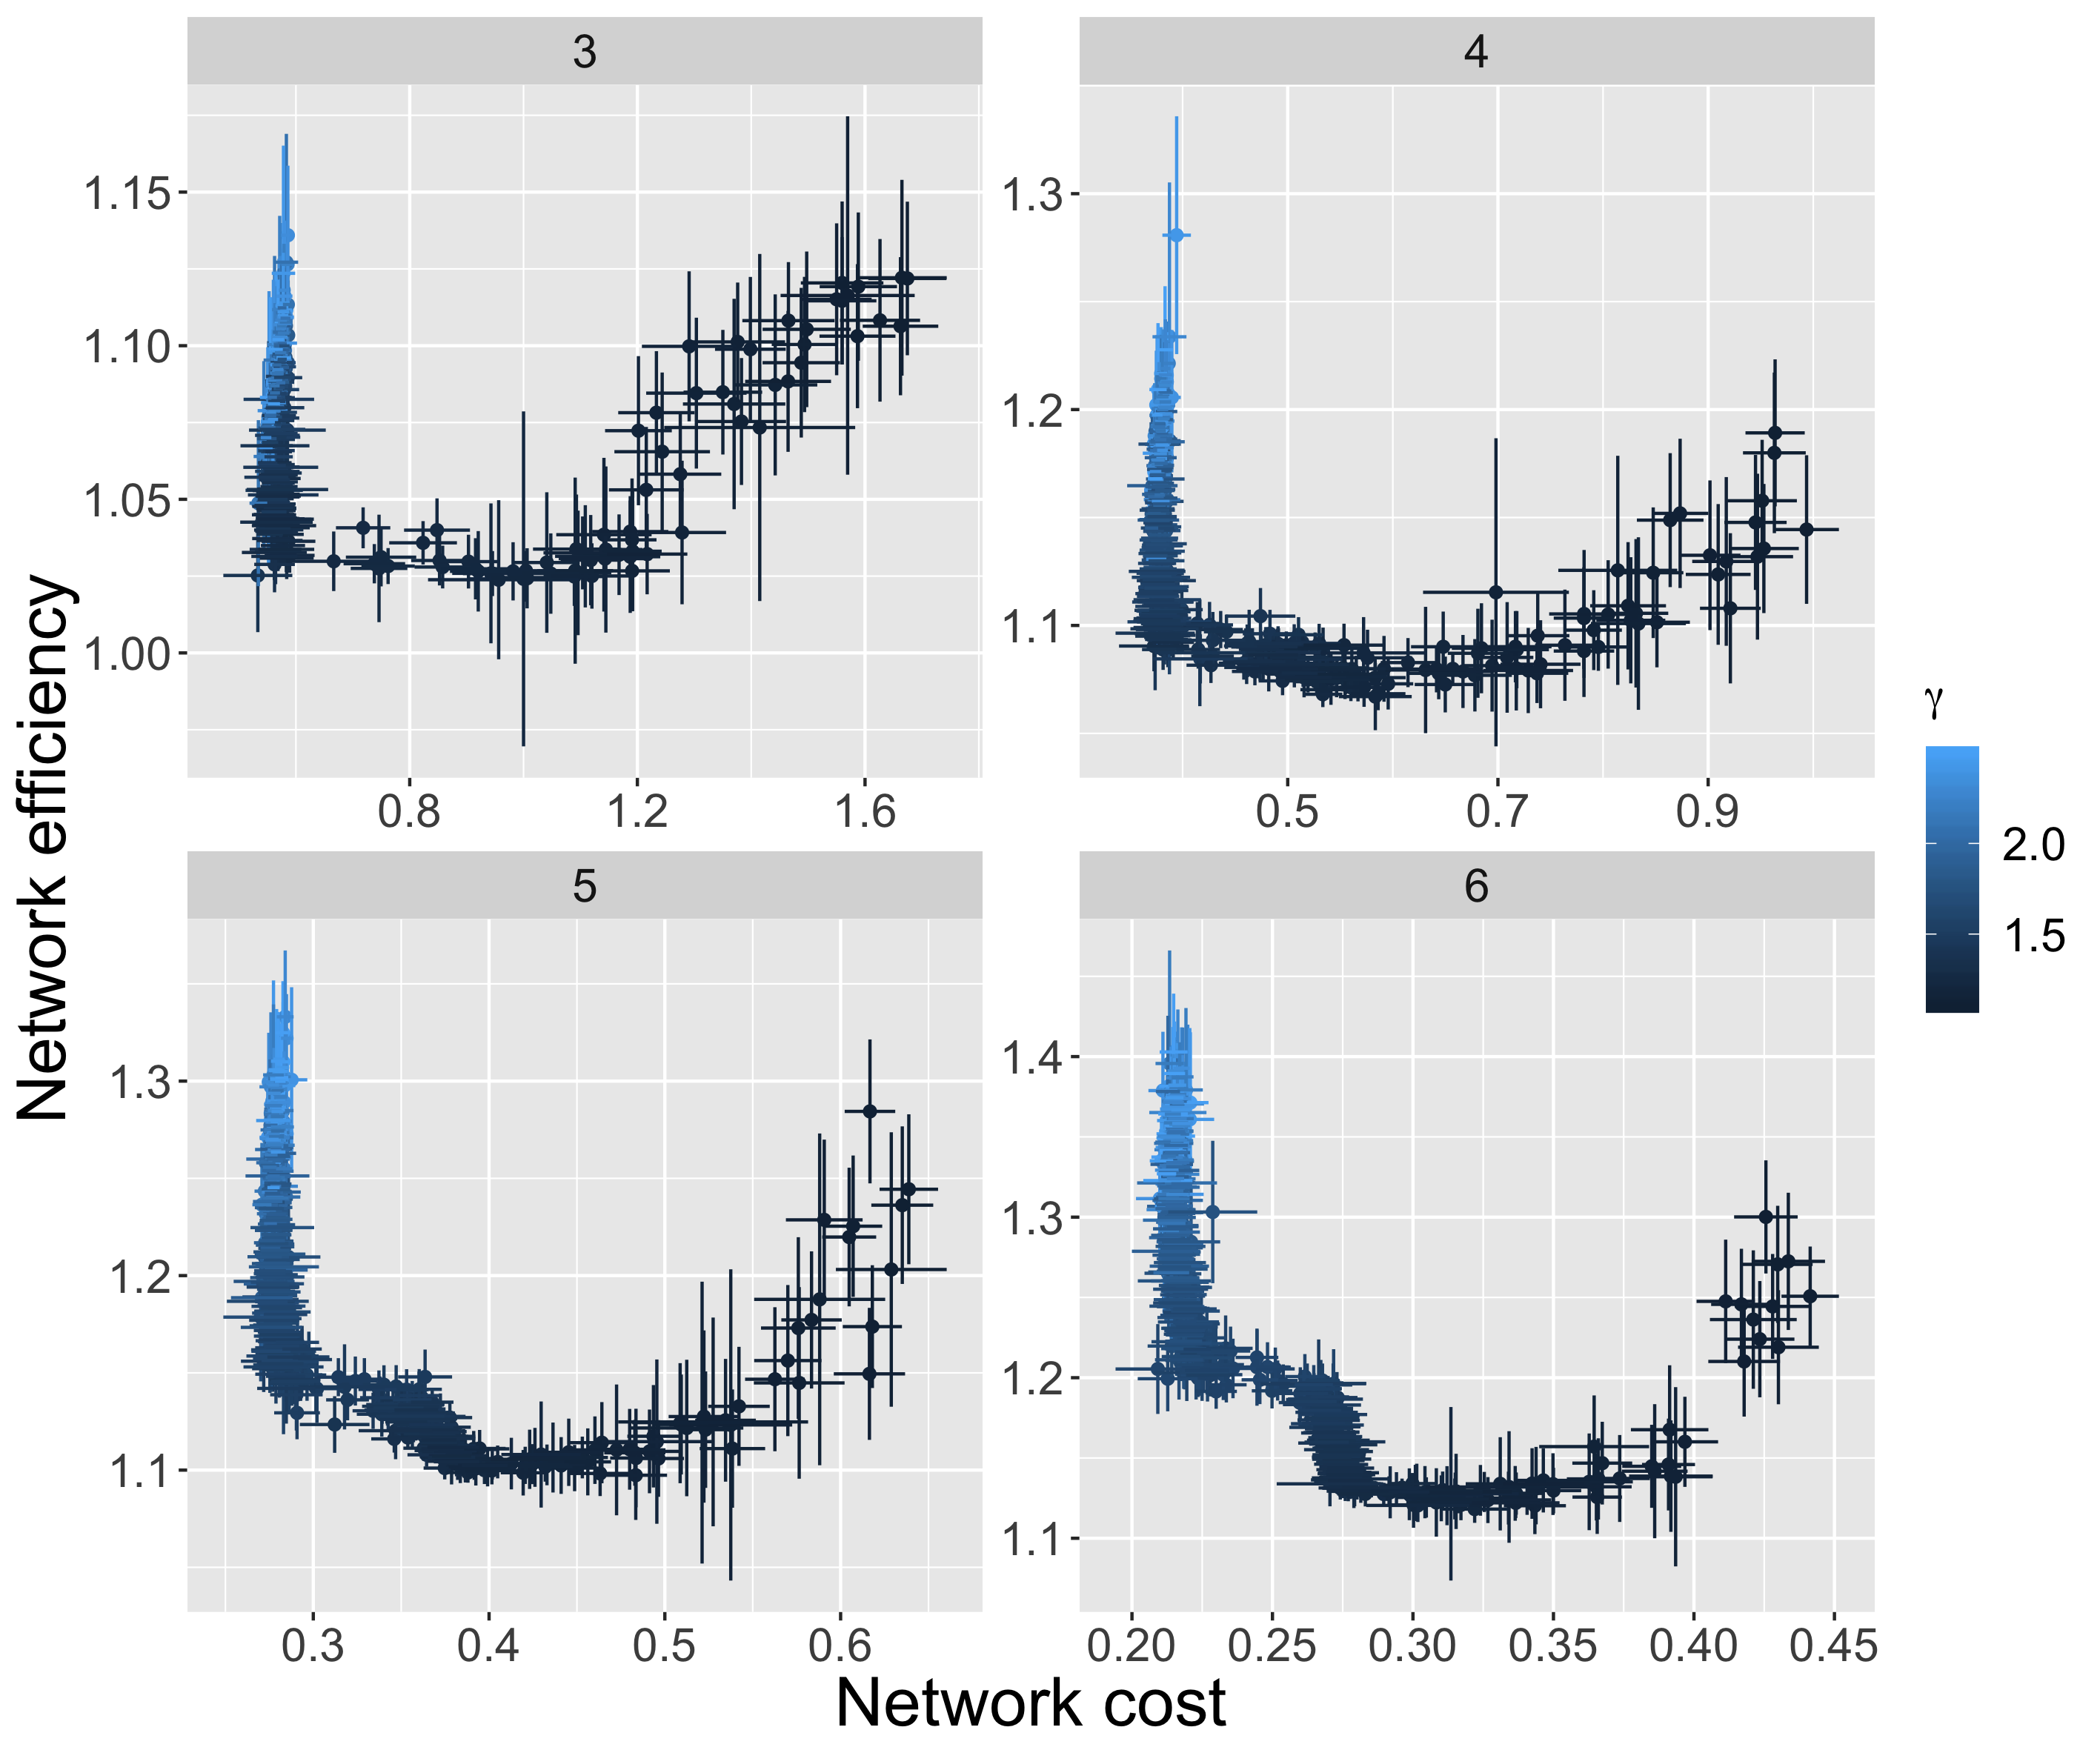
\includegraphics[width=0.5\textwidth]{figures/pareto_cost-speed_facetCenterNumber_withgaussianCI.png}

}


\sframe{Indicateurs}{

\begin{itemize}
	\item Indicateurs de réseau :%Network indicators (fixed by the scenario and the replication), both contradictory objective for which the network generation heuristic finds a compromise :
	\begin{itemize}
		\item coût relatif%network relative cost : length of the network relative to the length of the full euclidian network between all centers
		\item performance \cite{banos2012towards}
	\end{itemize}
	\item Indicateurs de soutenabilité%Sustainability indicators (should be the objective of PSE / OSE / calibrations). Can be contradictory but not clear :
	\begin{itemize}
		\item évolution de l'accessibilité (performance, équité territoriale)%Evolution of the average accessibility between initial and final state
		\item congestion%Average congestion, approximated by the average weighted betweenness centrality (using stationary commuting flows between actives and employments)
	\end{itemize}
	\item Indicateurs de forme urbaine \cite{raimbault2018calibration}%Urban form indicators : four dimensions (moran, average distance, entropy, hierarchy)  for population and employments
\end{itemize}

}


\sframe{Sensibilité aux scenarios}{
  
  \centering
  
  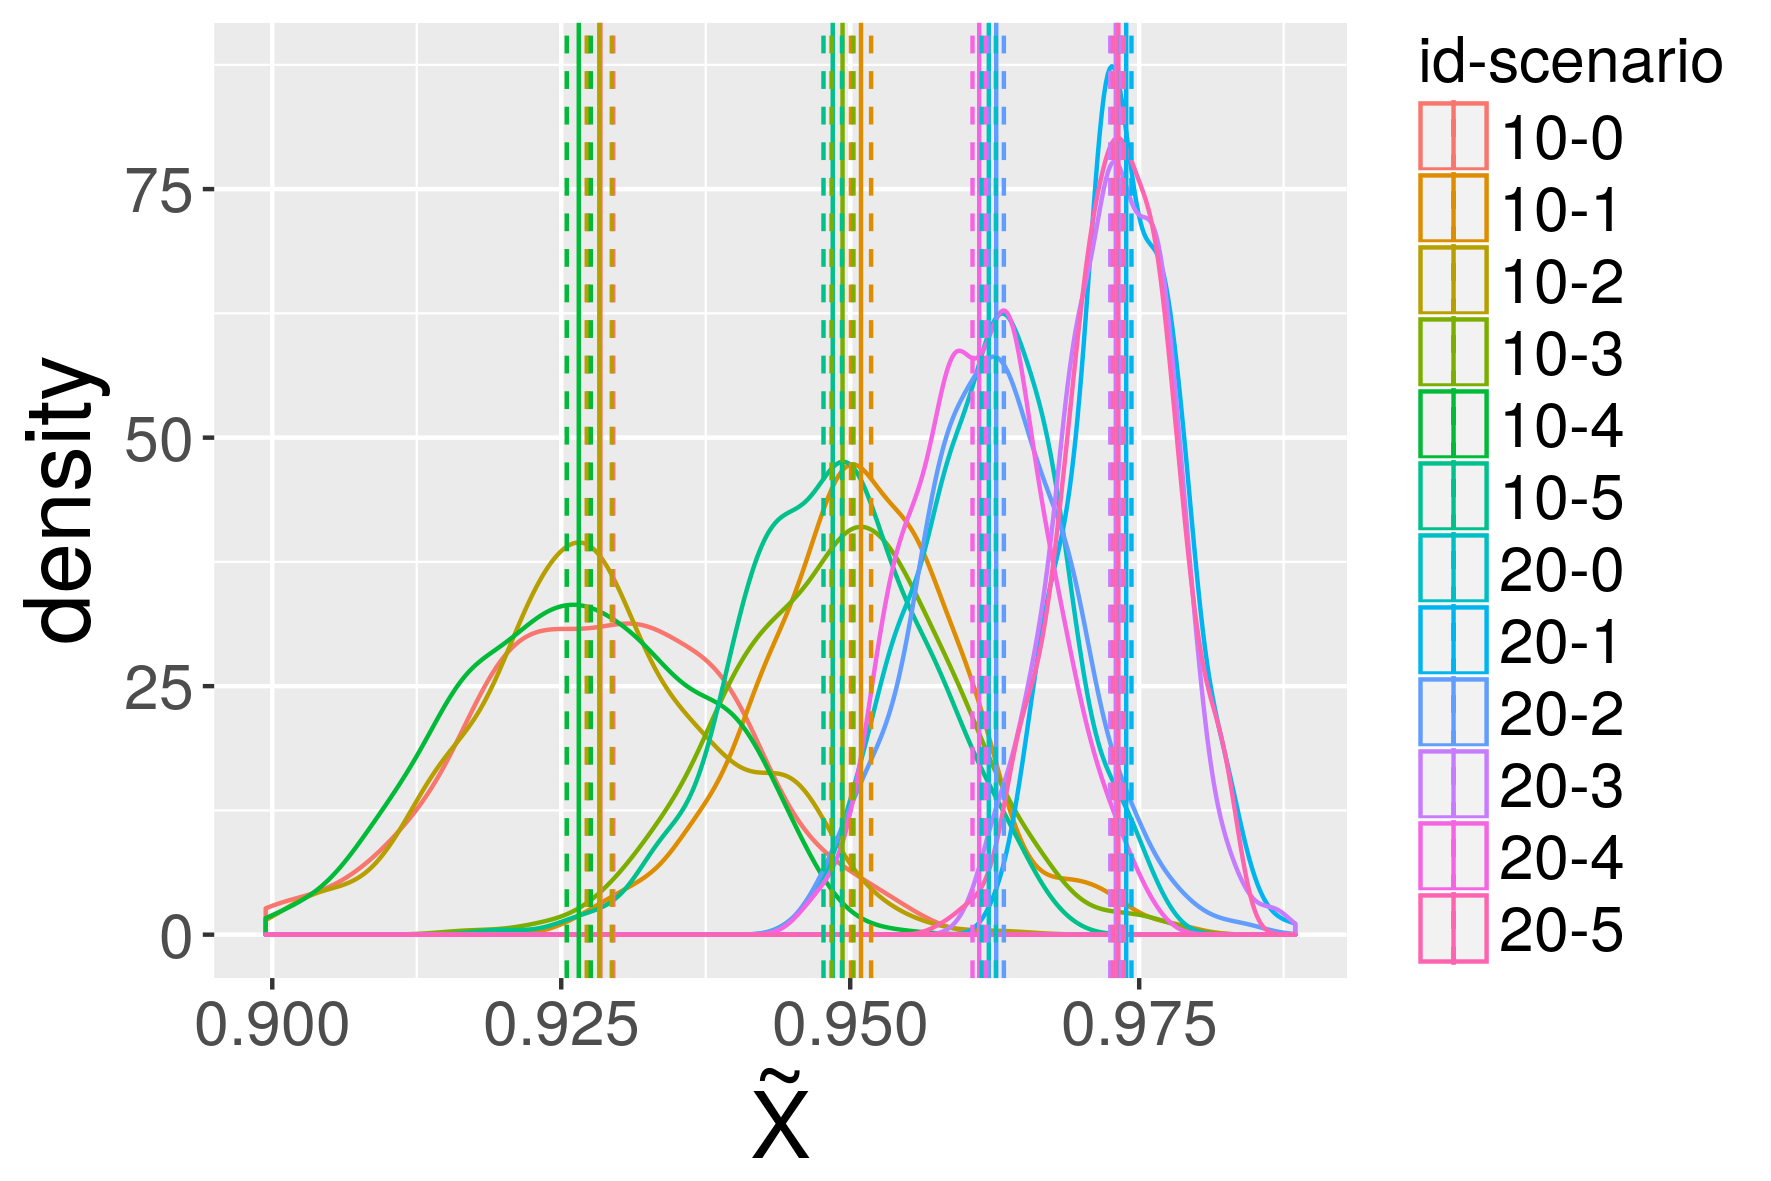
\includegraphics[width=0.8\textwidth]{figures/lutisens_sm.png}

	\medskip
	
	\footnotesize
	
	\begin{tabular}{|c|c|c|c|c|c|c|c|c|}
\hline
Parameter & $\beta$ & $\gamma_A$ & $\gamma_E$ & $\lambda$ & $\alpha$ & $v_0$ & scenario & residuals \\
\% variance & 0.11 & 0.68 & 0.46 & 45.71 & 2.22 & 23.12 & 7.27 & 20.43 \\
\hline
\end{tabular}


}


\sframe{Faits stylisés}{

\begin{itemize}
	\item ``\textit{more accessible areas are developed faster}'': $\rho\left[X_i,\Delta P_i\right] > 0$
	\item ``\textit{employments locate in highly accessible areas}'': $\rho\left[X_i,E_i\right] > 0$
	\item ``\textit{good access $\implies$ suburban dispersal $\implies$ longer trips}'': $\rho\left[X_i,t_i\right] > 0$ at the scale of a run, $\rho\left[\tilde{X},\alpha_A\right] > 0$ on repetitions
\end{itemize}

\medskip

$\rightarrow$ \textit{piste à explorer: validation ``qualitative'' des faits stylisés par l'intermédiaire de calibration et de recherche de diversité}

}

\sframe{Calibration / Optimisation}{

% OSE / sustainable points

1. \textit{Etant donné paramètres exogènes fixés (coût de l'énergie, système économique et comportements résidentiels), quelles structures urbaines/scénarios de transport sont optimaux pour les indicateurs de soutenabilité contradictoire congestion/accessibilité ? Et réciproquement ?}

$\rightarrow$ utilisation de calibration

\bigskip

2. \textit{Pour un niveau atteignable de soutenabilité, existe-t-il des scénarios distincts contingents pour l'atteindre ?}

$\rightarrow$ utilisation/test d'\textit{inverse problem method} (algorithme OSE)

}


\sframe{Modèle Dynamicity: recherche de diversité}{

% + reduction de dimension ?


Parameters correspond to a perturbation of the discrete choice model coefficients, i.e. a $\vec{\Delta \beta}_c$ such that the model is run with $U_{i,c} = (\vec{\beta}_{c} + \vec{\Delta \beta}_c )\cdot \vec{X}_{i,c}$.

Boundaries are fixed depending on the confidence interval obtained during the estimation of the multinomial logit model: if $\vec{\beta}_{c} = (\beta_{c,j})_j$ et $\beta_{c,j} \in \left[\beta_{c,j}^- ; \beta_{c,j}^+\right]$, we then take

\[
\left|\Delta \beta_{c,j}\right| \in \delta_{c,j} \cdot (\beta_{c,j}^+ - \beta_{c,j}^-)
\]

$\rightarrow$ PSE algorithm on $\delta_{c,j}$

}



\sframe{Modèle dynamicity}{

Convergence du nombre de patterns en très haute dimension ?

% question de la dimensionalité

\medskip

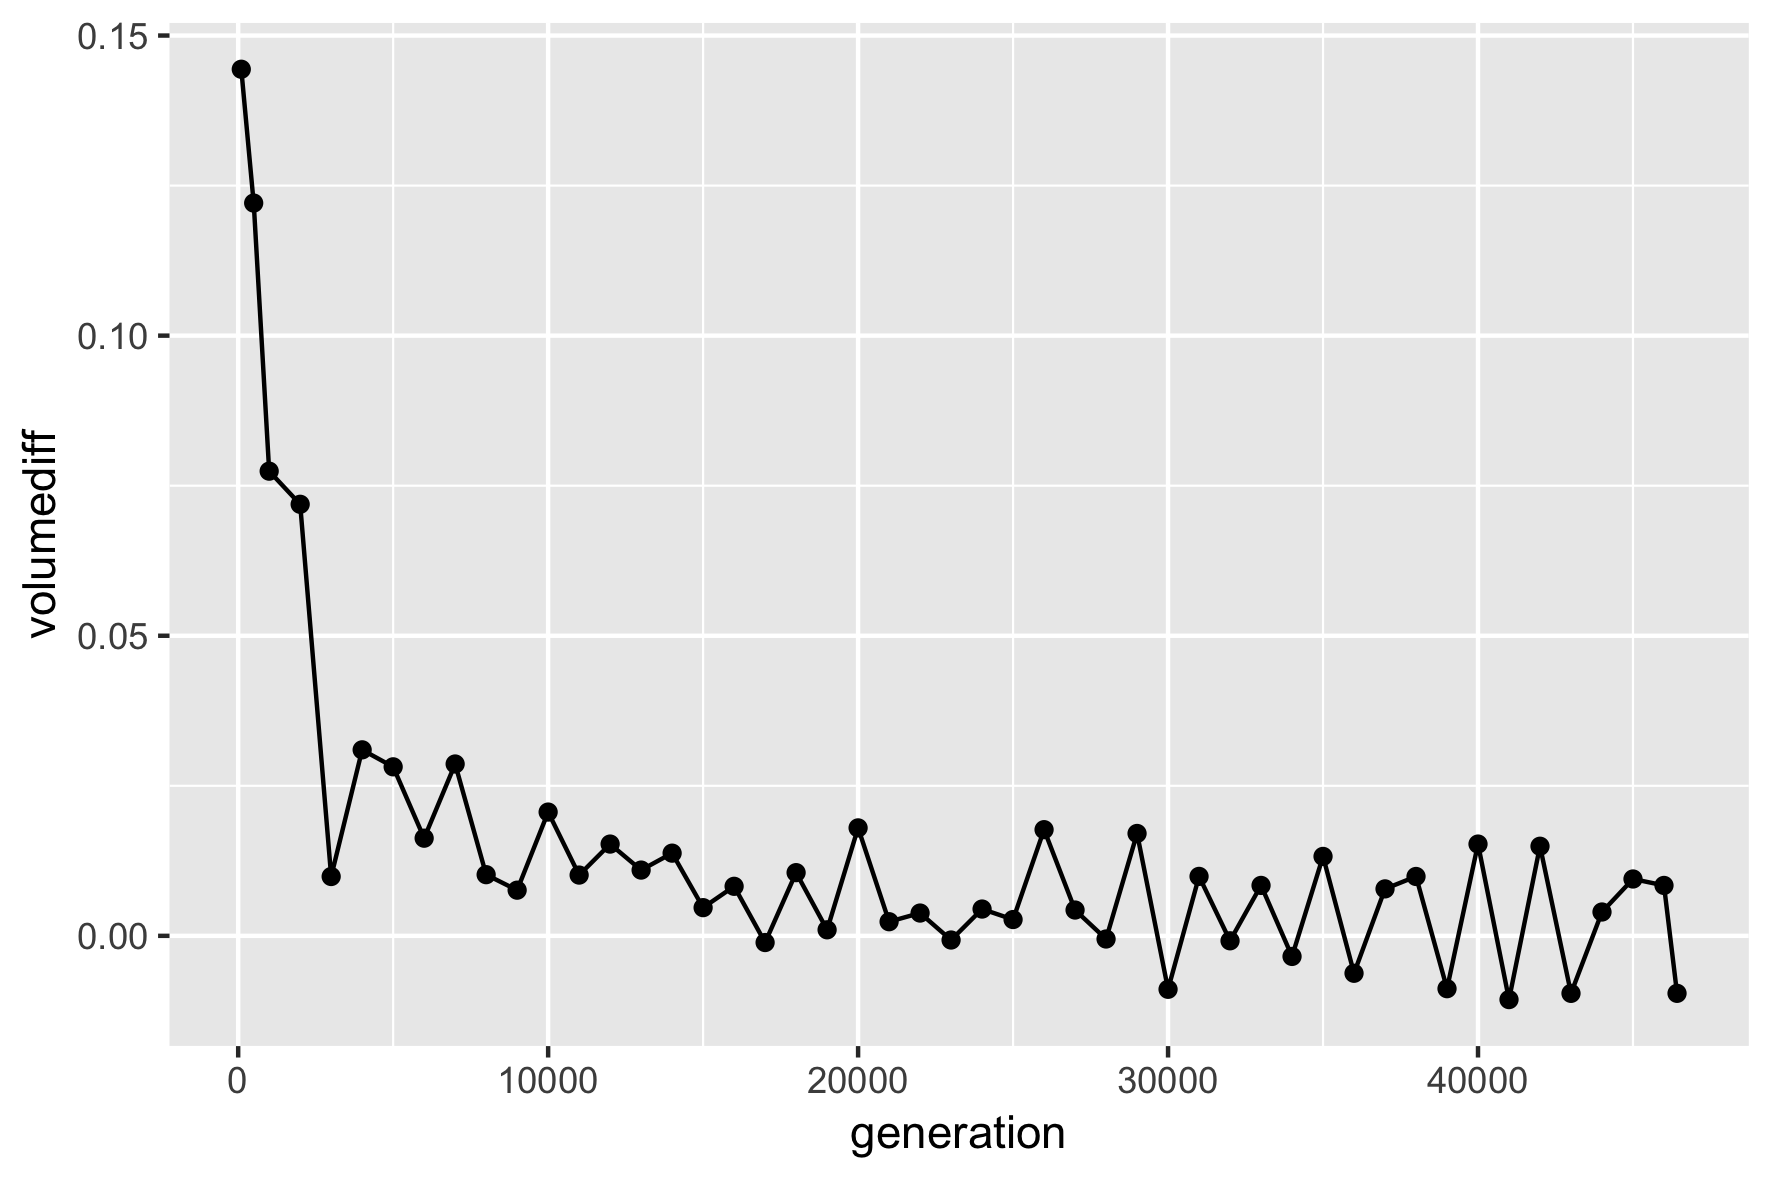
\includegraphics[width=0.5\textwidth]{figures/hypervolumediff.png}
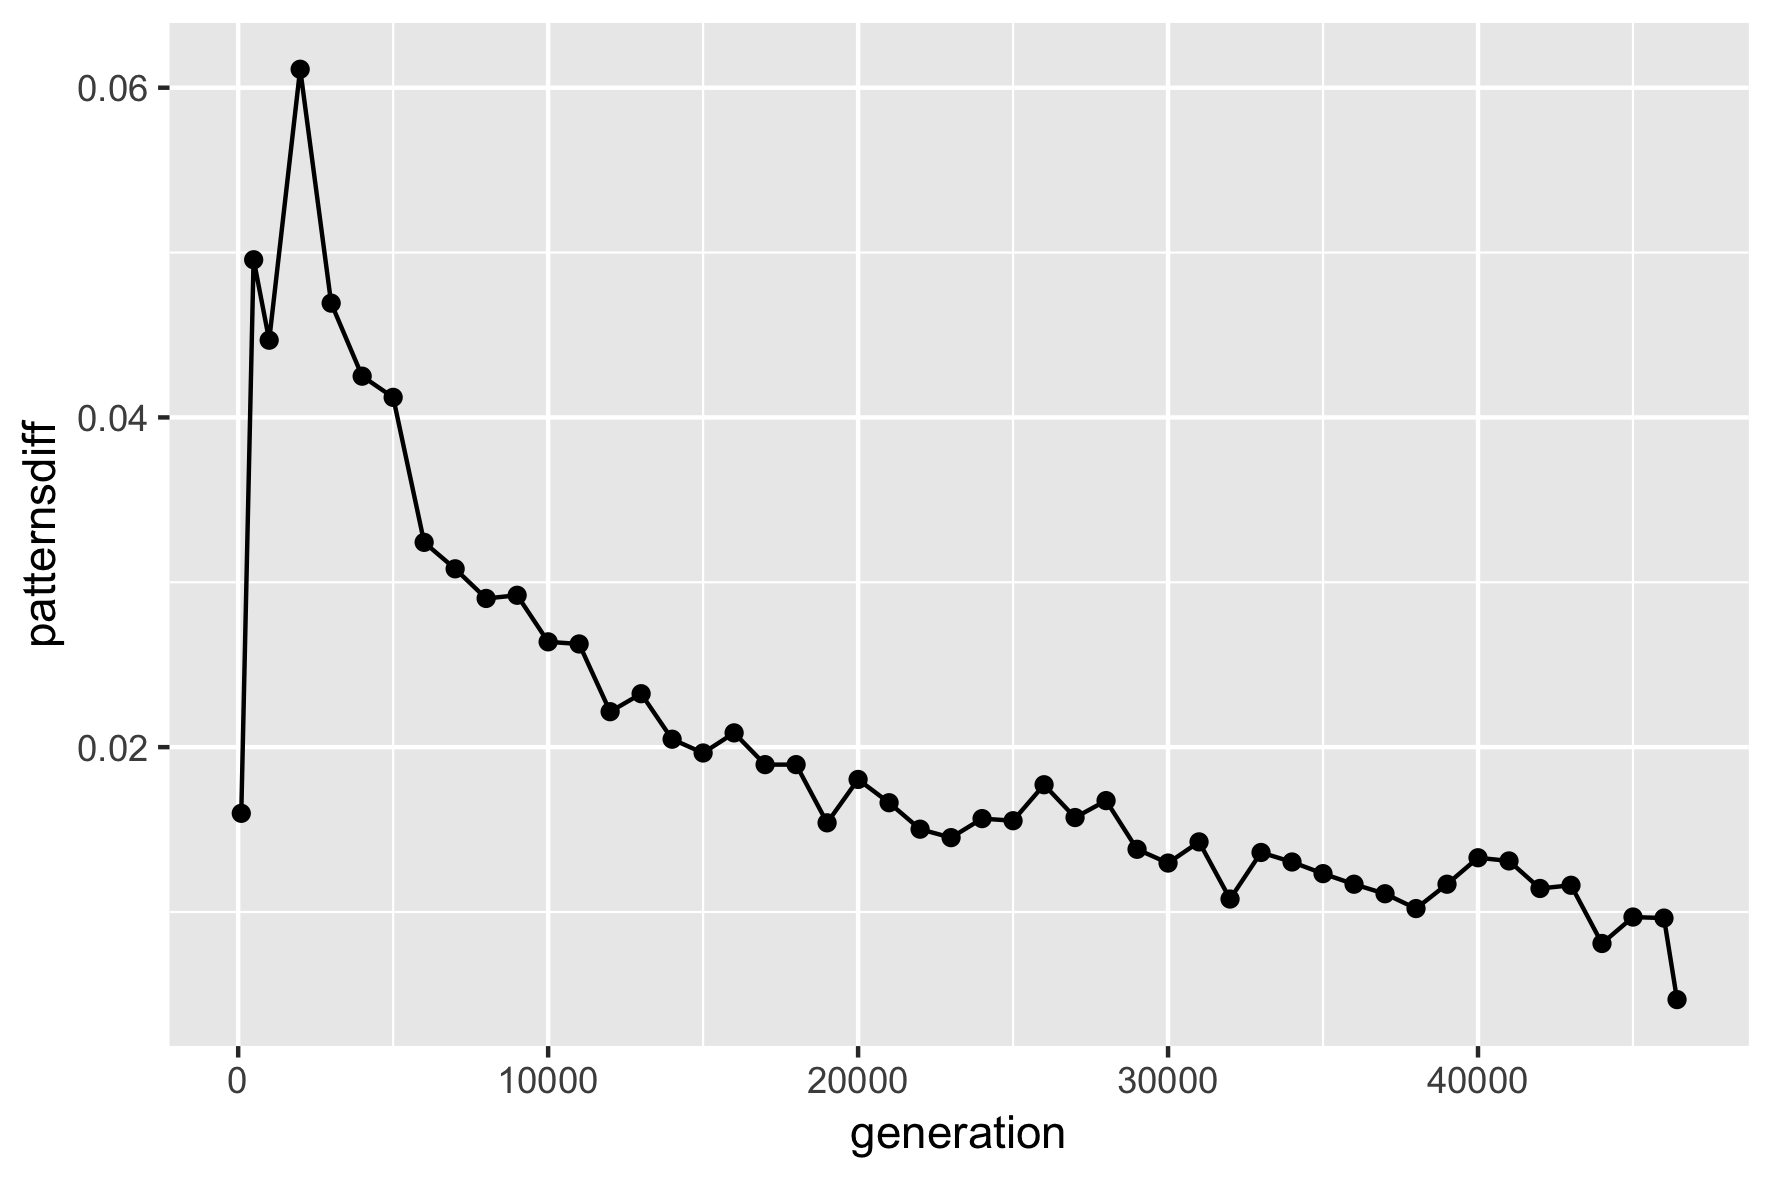
\includegraphics[width=0.5\textwidth]{figures/patternsdiff.png}

\medskip

$\rightarrow$ dimension effective : $\simeq 4$ à 80\% de variance (24 dimensions) 

$\rightarrow$ réduction de dimension couplée à PSE ?

}

\sframe{Développements}{

\begin{itemize}
	\item Sensitivity to the network: application of the method developed by \cite{cottineau2017initial} to test the sensitivity to network topology and/or missing data
    \item Sensitivity to the traffic model used: for example compare the betweenness-based currently implemented to a SUE \cite{wardrop1952some}
    \item Sensitivity to the synthetic population generator: couple with the analysis of the upstream model
    \item Temporal calibration on real trajectories ? historical data iris: partial dynamical calibration on intermediate aggregations 
\end{itemize}

}





\sframe{Conclusion}{

$\rightarrow$ des modèles très data-driven et appliqués en pratique, mais loin d'être systématiquement validés : enjeux significatifs pour des politiques evidence-based %First step towards systematic benchmarks and multi-modeling. \textbf{Need for more systematic model exploration.} % model coupling / benchmarking


$\rightarrow$ vers des modèles intégrés, interdisciplinaires et multi-échelles%Model integration and multi-scalarity ? \textbf{Need for more integrated models.}


$\rightarrow$ enjeux crucial pour les transitions durables (l'urbain et les territoires négligés des travaux mainstream sur le changement climatique) %Multiple perspectives on urban systems ? \textbf{Need for more interdisciplinarity.}
%\textbf{Open repository} at \texttt{https://github.com/JusteRaimbault/UrbanGrowth}\\\smallskip

\bigskip

\textbf{Acknowledgments}: thanks to the \textit{EGI} for access to the infrastructure.
}






\sframe{Reserve slides}{
\centering
\Large
\textbf{Reserve Slides}
}


%%%%%%%%%%%%%%%%%%%%%
\begin{frame}[allowframebreaks]
\frametitle{References}
\bibliographystyle{apalike}
\bibliography{biblio}
\end{frame}
%%%%%%%%%%%%%%%%%%%%%%%%%%%%




\end{document}









